\section{FORESEE}
\label{res:tinydas}


\subsection{Experiment \rnum{1}: Model training and Reconstruction}

\begin{table}[!htbp]
    \centering
    \small
    \setlength{\tabcolsep}{10pt}
    \begin{tabular}{l S[table-format=1.3e-1] S[table-format=1.3] S[table-format=1.3] S[table-format=1.3]}
        \toprule
        \rowcolor{gray!20}
        \textbf{Metric} & {\textbf{AE}} & {\textbf{$\beta$-VAE}} & {\textbf{CAE}} & {\textbf{$\beta$-CVAE}} \\
        \midrule
        Best Train loss & 1.3e-6 & 0.032 & 0.038 & 0.029 \\
        \rowcolor{gray!10}
        Best Validation loss & 1.3e-6 & 0.032 & 0.038 & 0.029 \\
        Epochs before stop & 6 & 20 & 15 & 15 \\
        \rowcolor{gray!10}
        Model Sizes & {\SI{10.240}{\giga\byte}} & {\SI{11.200}{\giga\byte}} & {\textbf{\SI{0.18}{\mega\byte}}} & {\textbf{\SI{47.06}{\mega\byte}}} \\
        \bottomrule
    \end{tabular}
    \caption{Comparison of Autoencoder Performance}
    \label{tab:modelresinfo}
    \smallskip
    \small{*The reconstruction error is the sum of all reconstruction errors across all batches.}
\end{table}

\begin{figure}[!h]
    \centering
    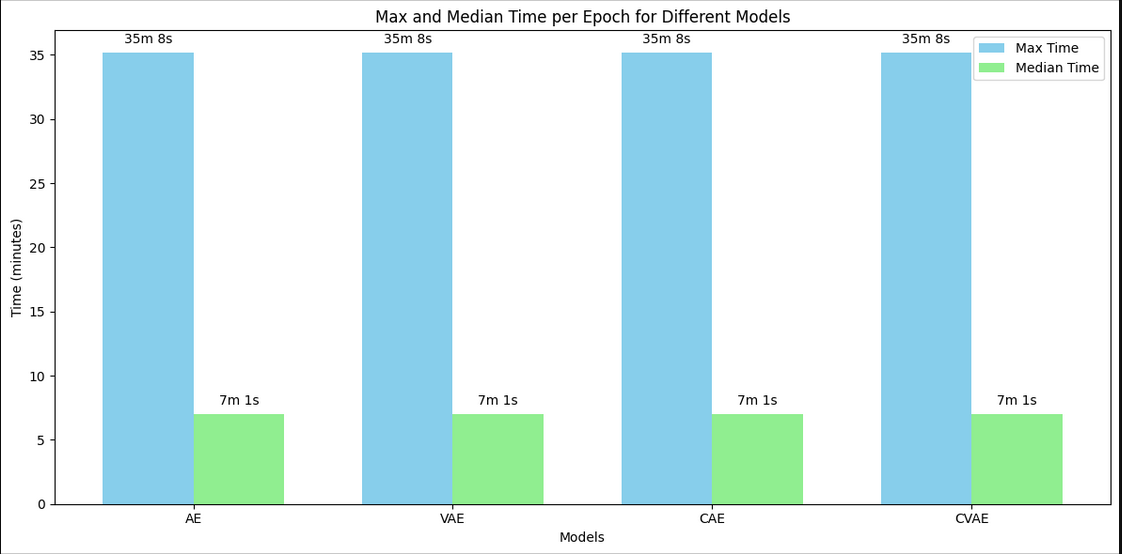
\includegraphics[scale=0.4]{figures/time.png}
    \caption{Training times}
    \label{fig:traintimes}
\end{figure}



\subsubsection{Loss Values}

\begin{figure}[!h]
  \centering
  \begin{subfigure}[t]{.6\textwidth}
    \centering
    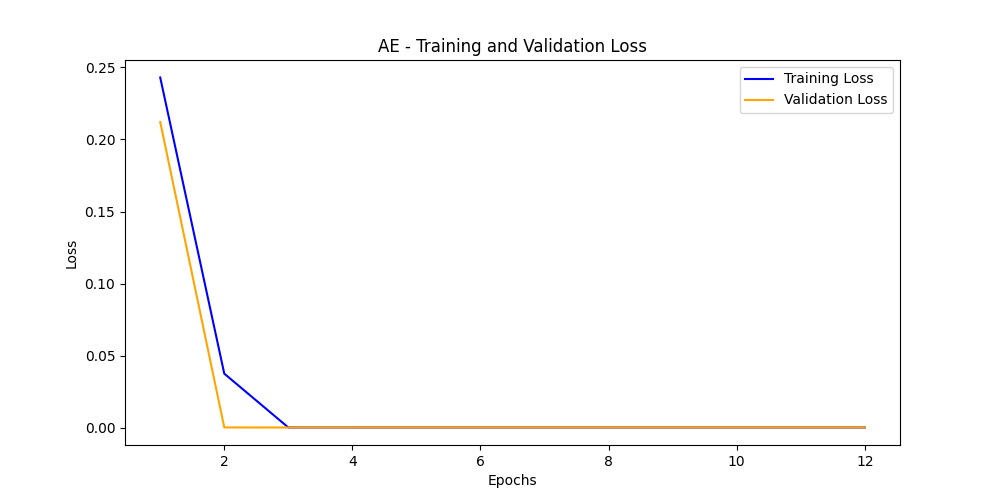
\includegraphics[width=\linewidth]{figures/losses/ae.png}
    \caption{AE}
  \end{subfigure}
  \hfill
  \begin{subfigure}[t]{.6\textwidth}
    \centering
    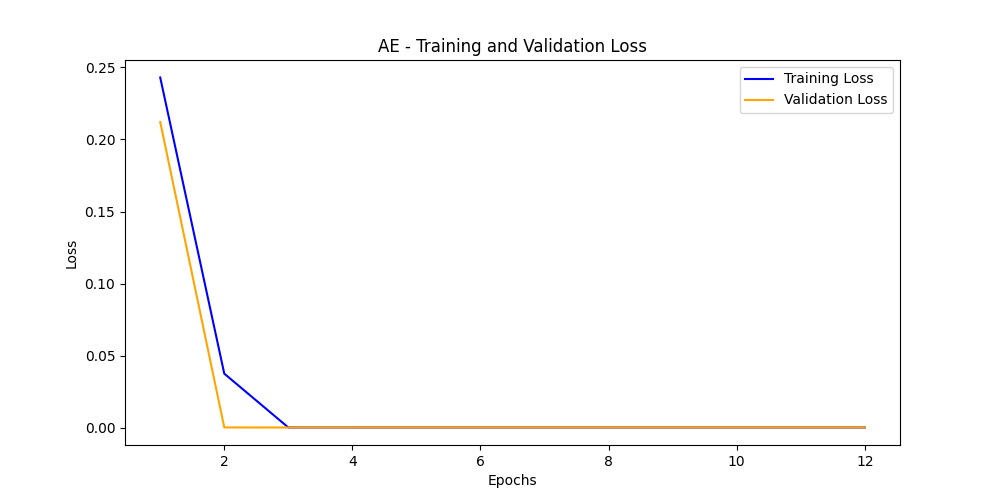
\includegraphics[width=\linewidth]{figures/losses/ae.png}
    \caption{CAE}
  \end{subfigure}
  
  \vspace{1cm}
  
  \begin{subfigure}[t]{.6\textwidth}
    \centering
    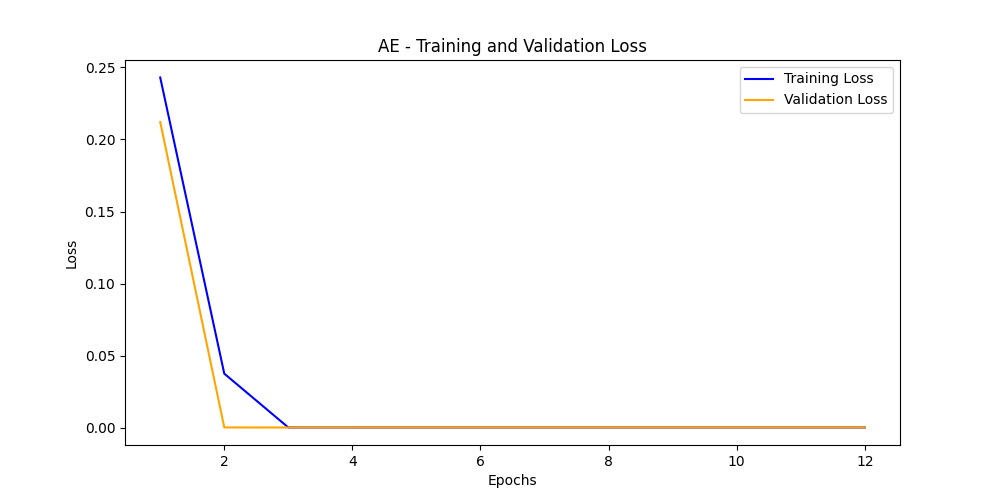
\includegraphics[width=\linewidth]{figures/losses/ae.png}
    \caption{$\beta$-VAE}
  \end{subfigure}
  \hfill
  \begin{subfigure}[t]{.6\textwidth}
    \centering
    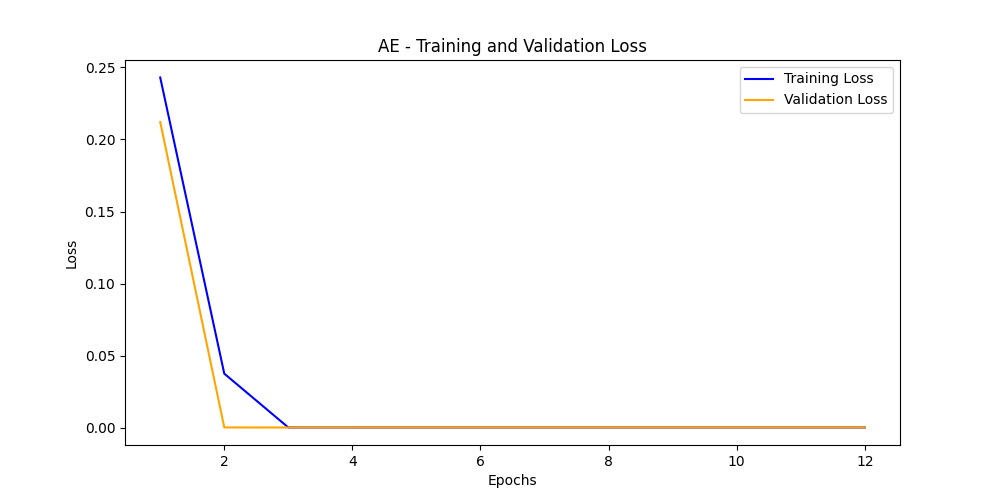
\includegraphics[width=\linewidth]{figures/losses/ae.png}
    \caption{$\beta$-CVAE}
  \end{subfigure}
  \label{fig:losses}
  \caption{Train and Validation Loss per epoch}
\end{figure}



\subsubsection{Reconstruction Capabiltites}

\begin{figure}[!h]
    \centering    
    % Row 0 (Image Names)
    \begin{subfigure}{0.33\textwidth}
        \centering
        \textbf{2019 04 15 - 03 17 35}
    \end{subfigure}%
    \hfill
    \begin{subfigure}{0.33\textwidth}
        \centering
        \textbf{2019 04 15 - 03 17 50}
    \end{subfigure}%
    \hfill
    \begin{subfigure}{0.33\textwidth}
        \centering
        \textbf{2019 04 15 - 03 17 55}
    \end{subfigure}
    
    \vspace{1em}
    
    % Row 1 (Original)
    \begin{subfigure}{0.33\textwidth}
        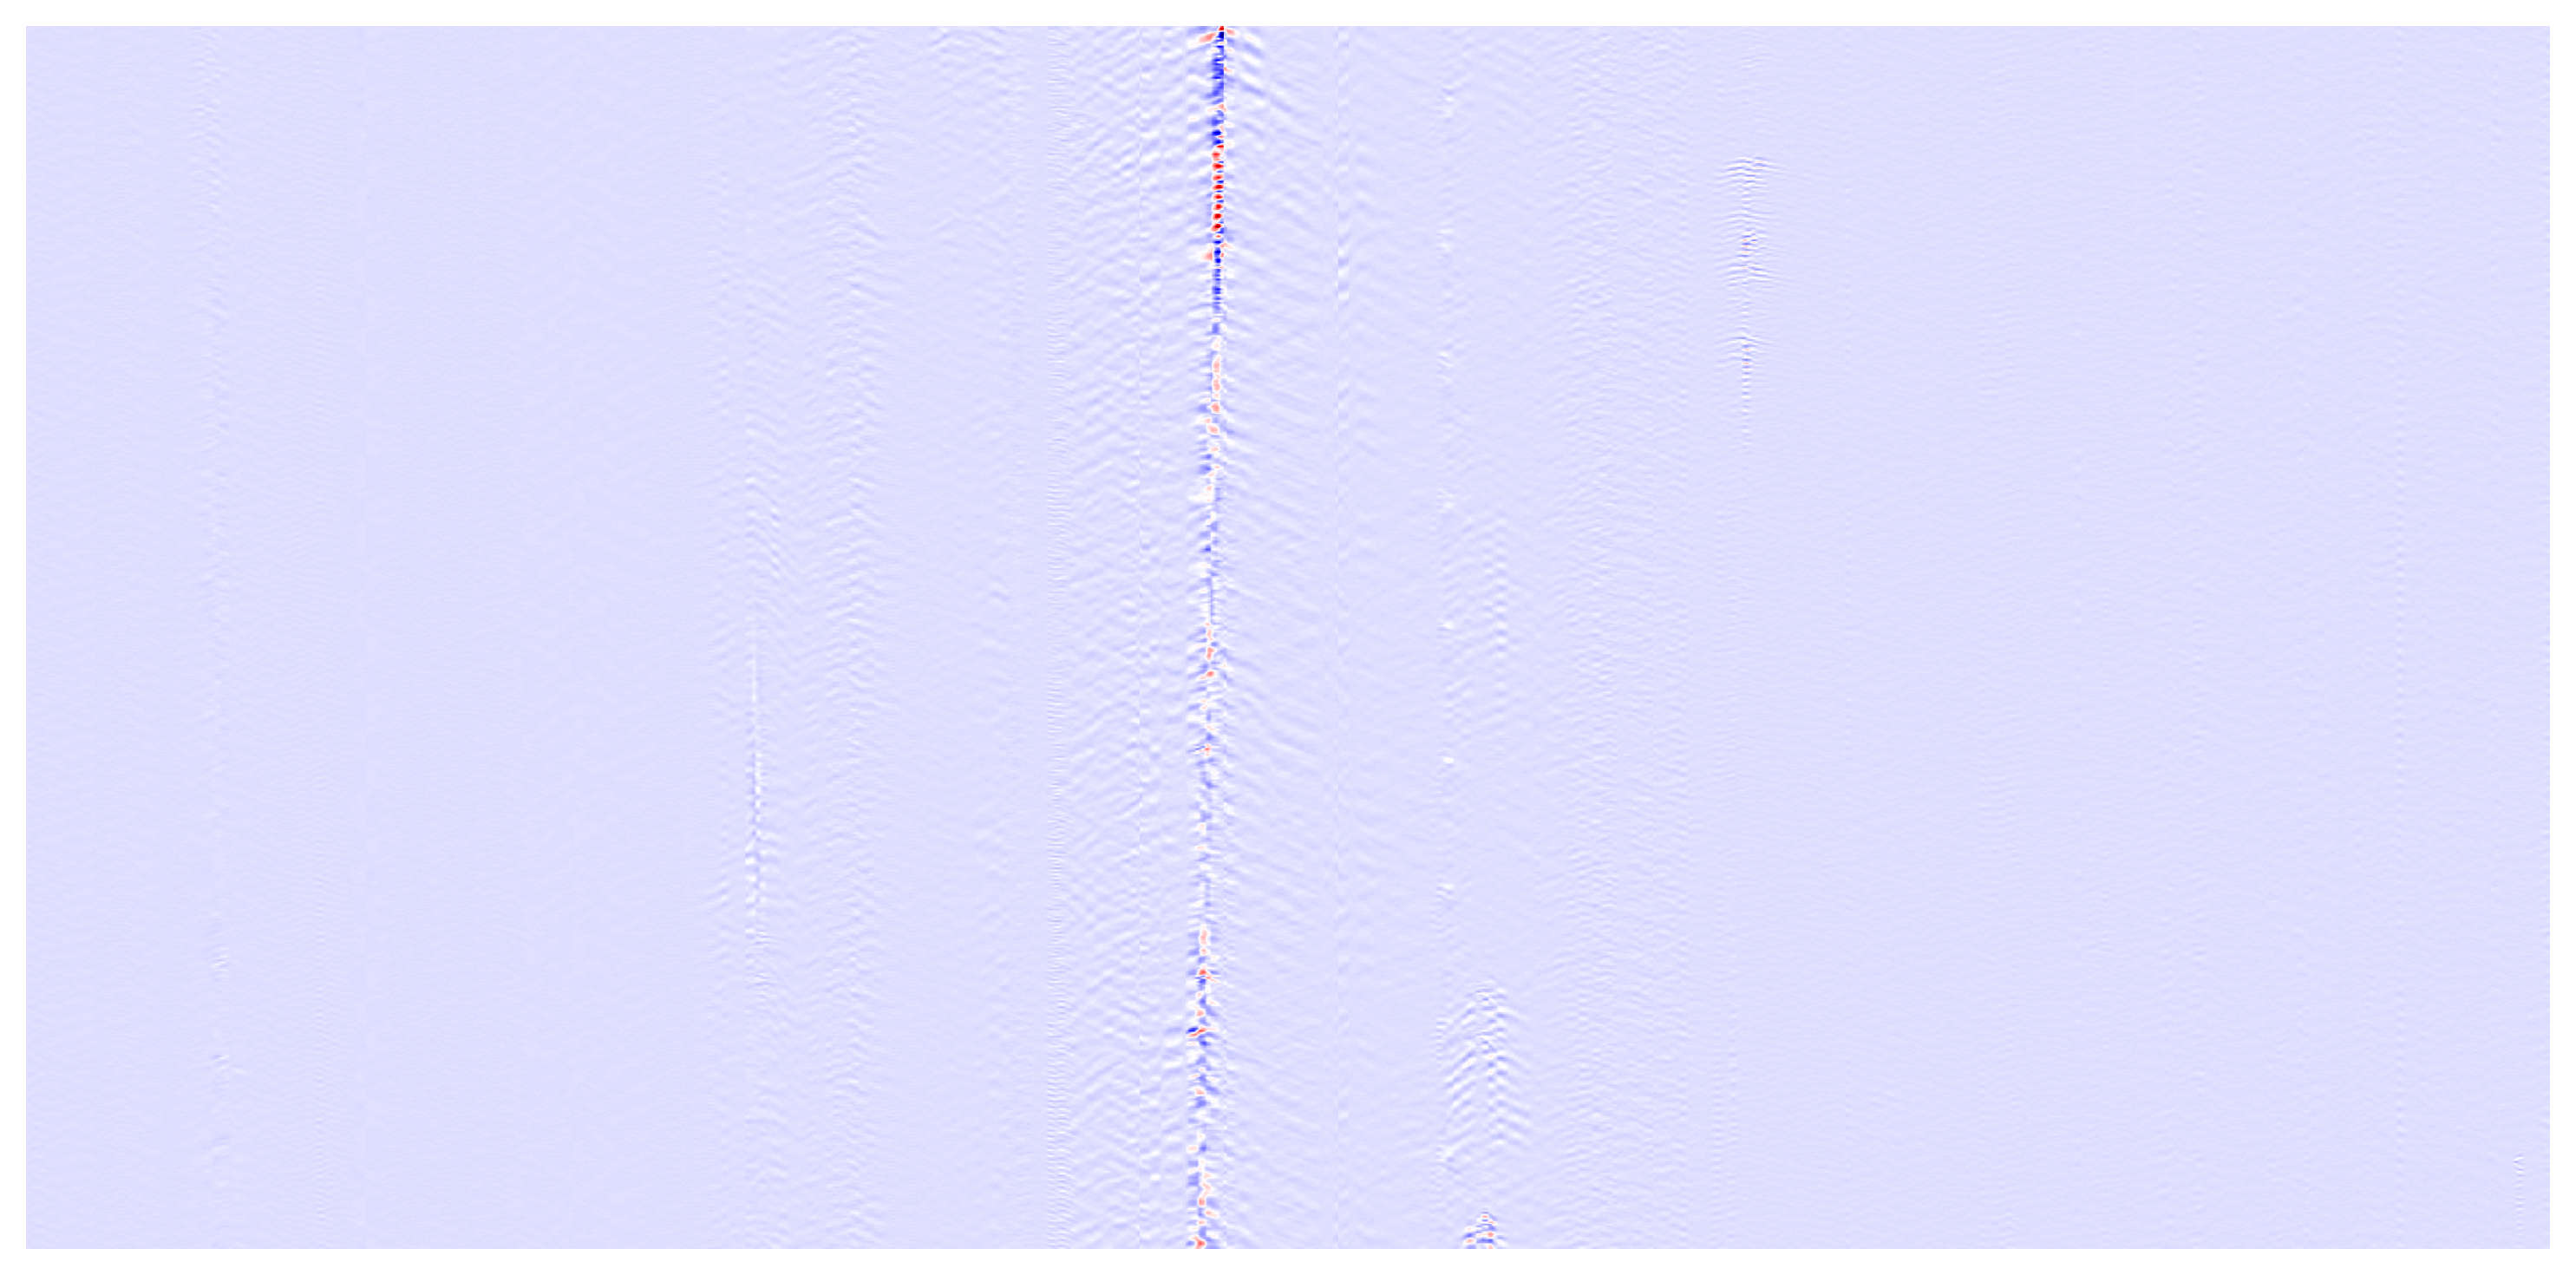
\includegraphics[width=\textwidth]{figures/anomalies/before/20190415_031735.png}
    \end{subfigure}%
    \hfill
    \begin{subfigure}{0.33\textwidth}
        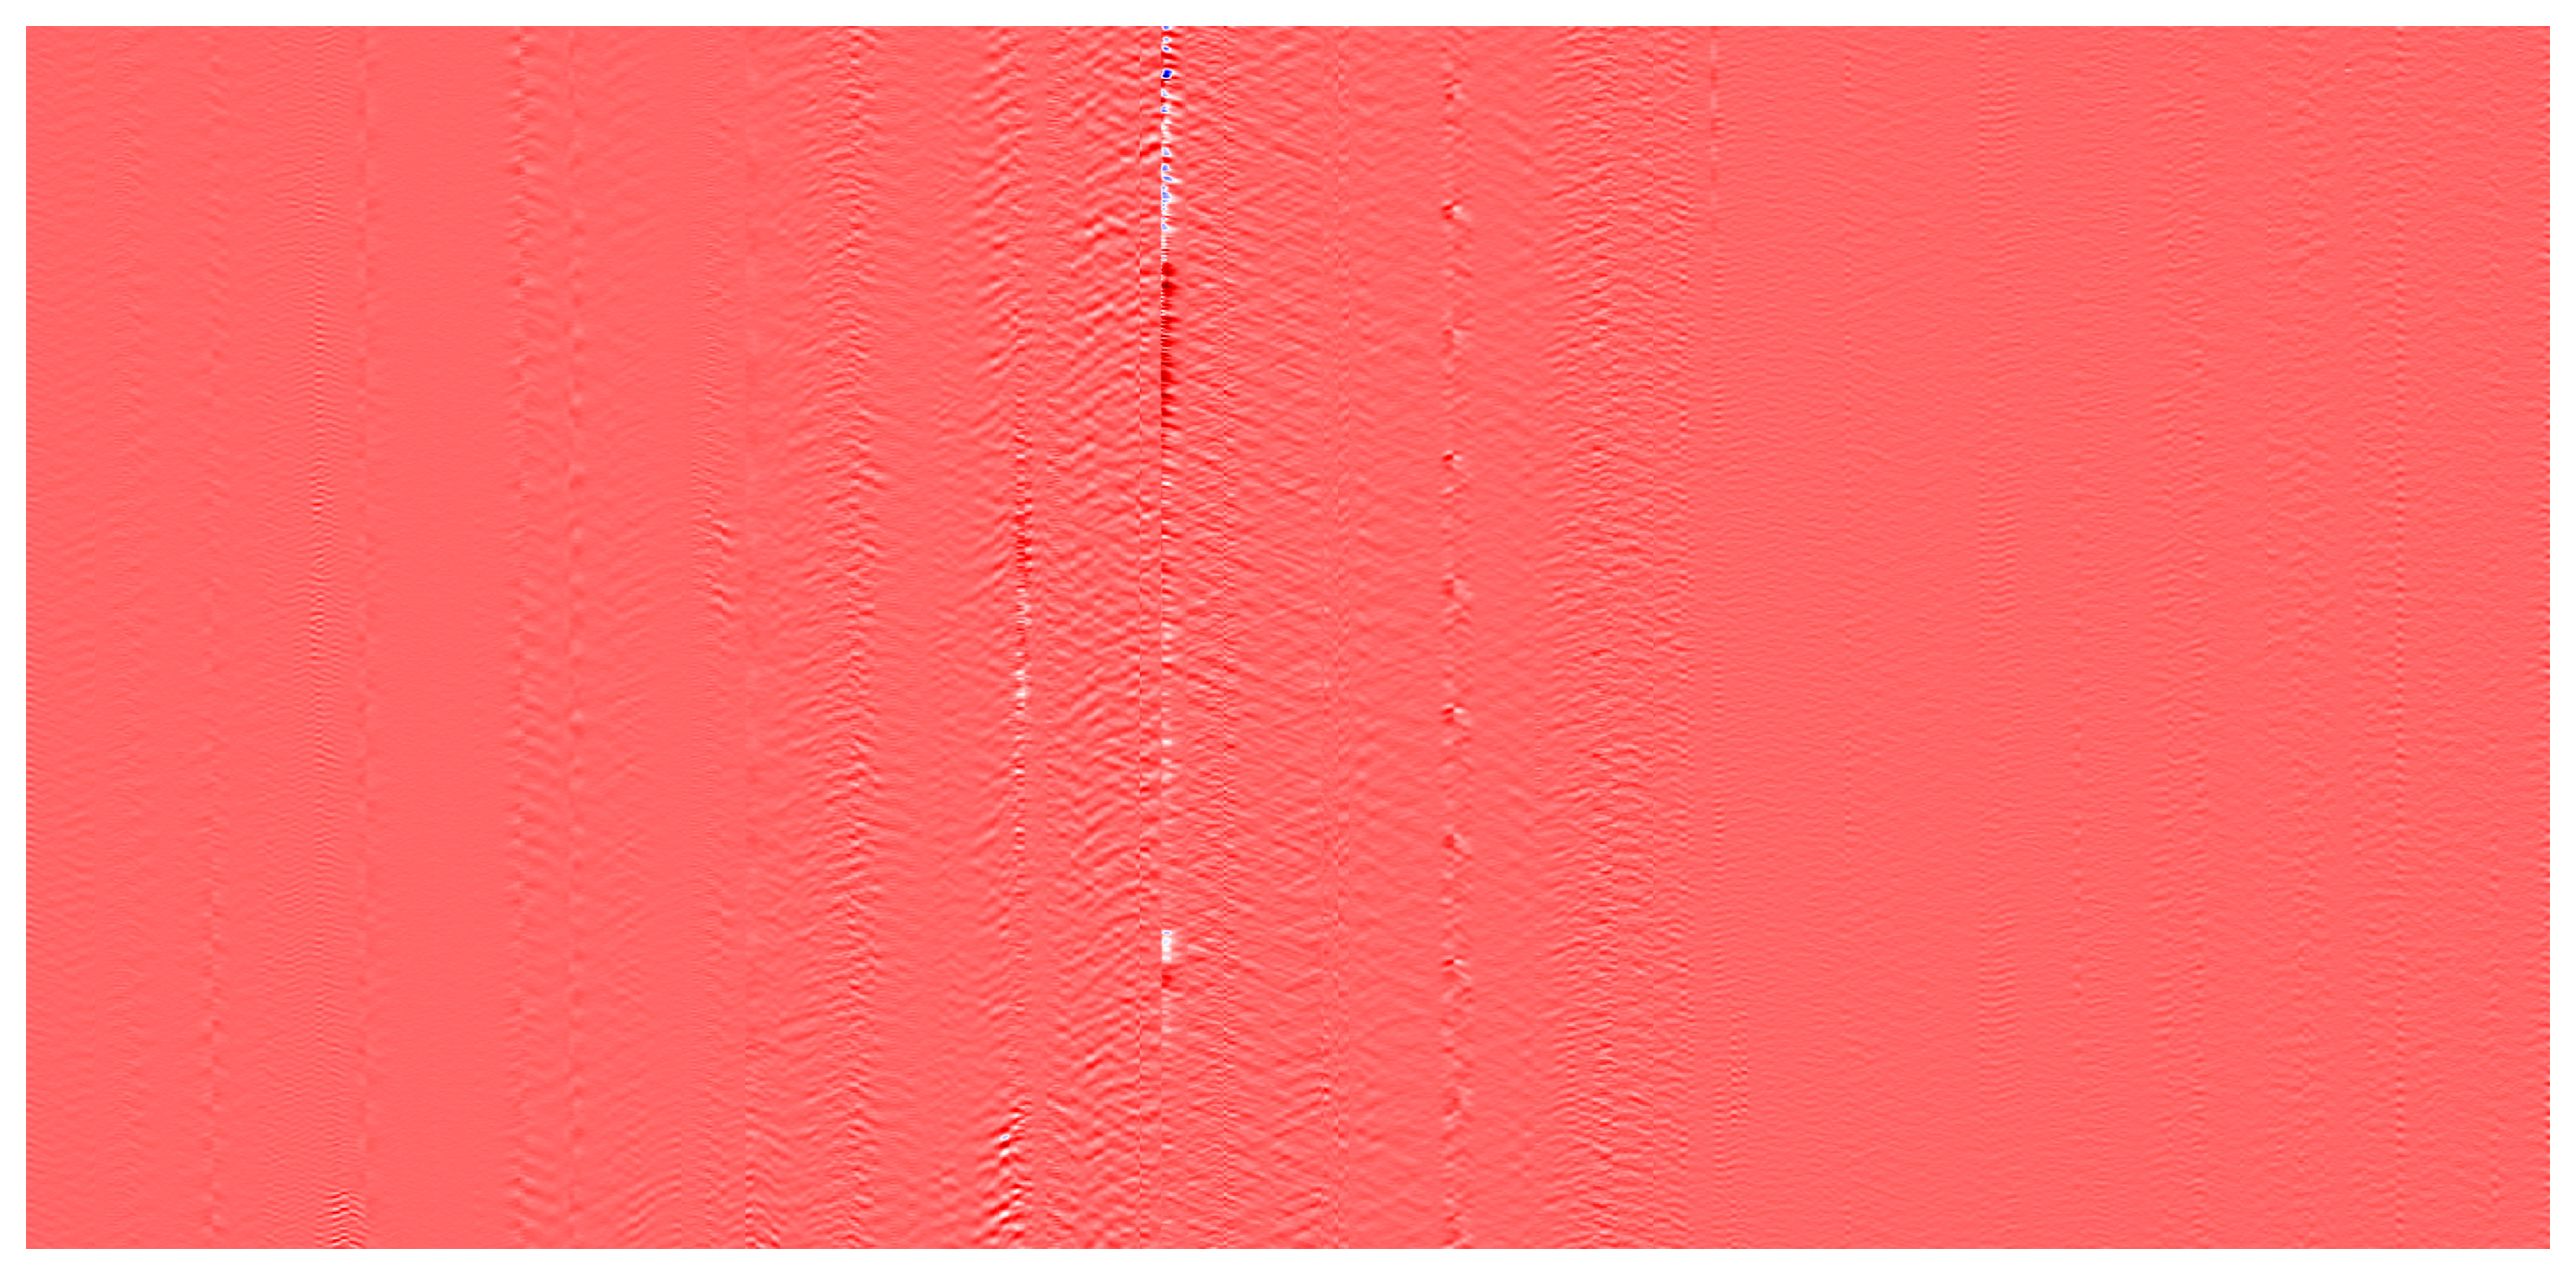
\includegraphics[width=\textwidth]{figures/anomalies/before/20190415_031750.png}
    \end{subfigure}%
    \hfill
    \begin{subfigure}{0.33\textwidth}
        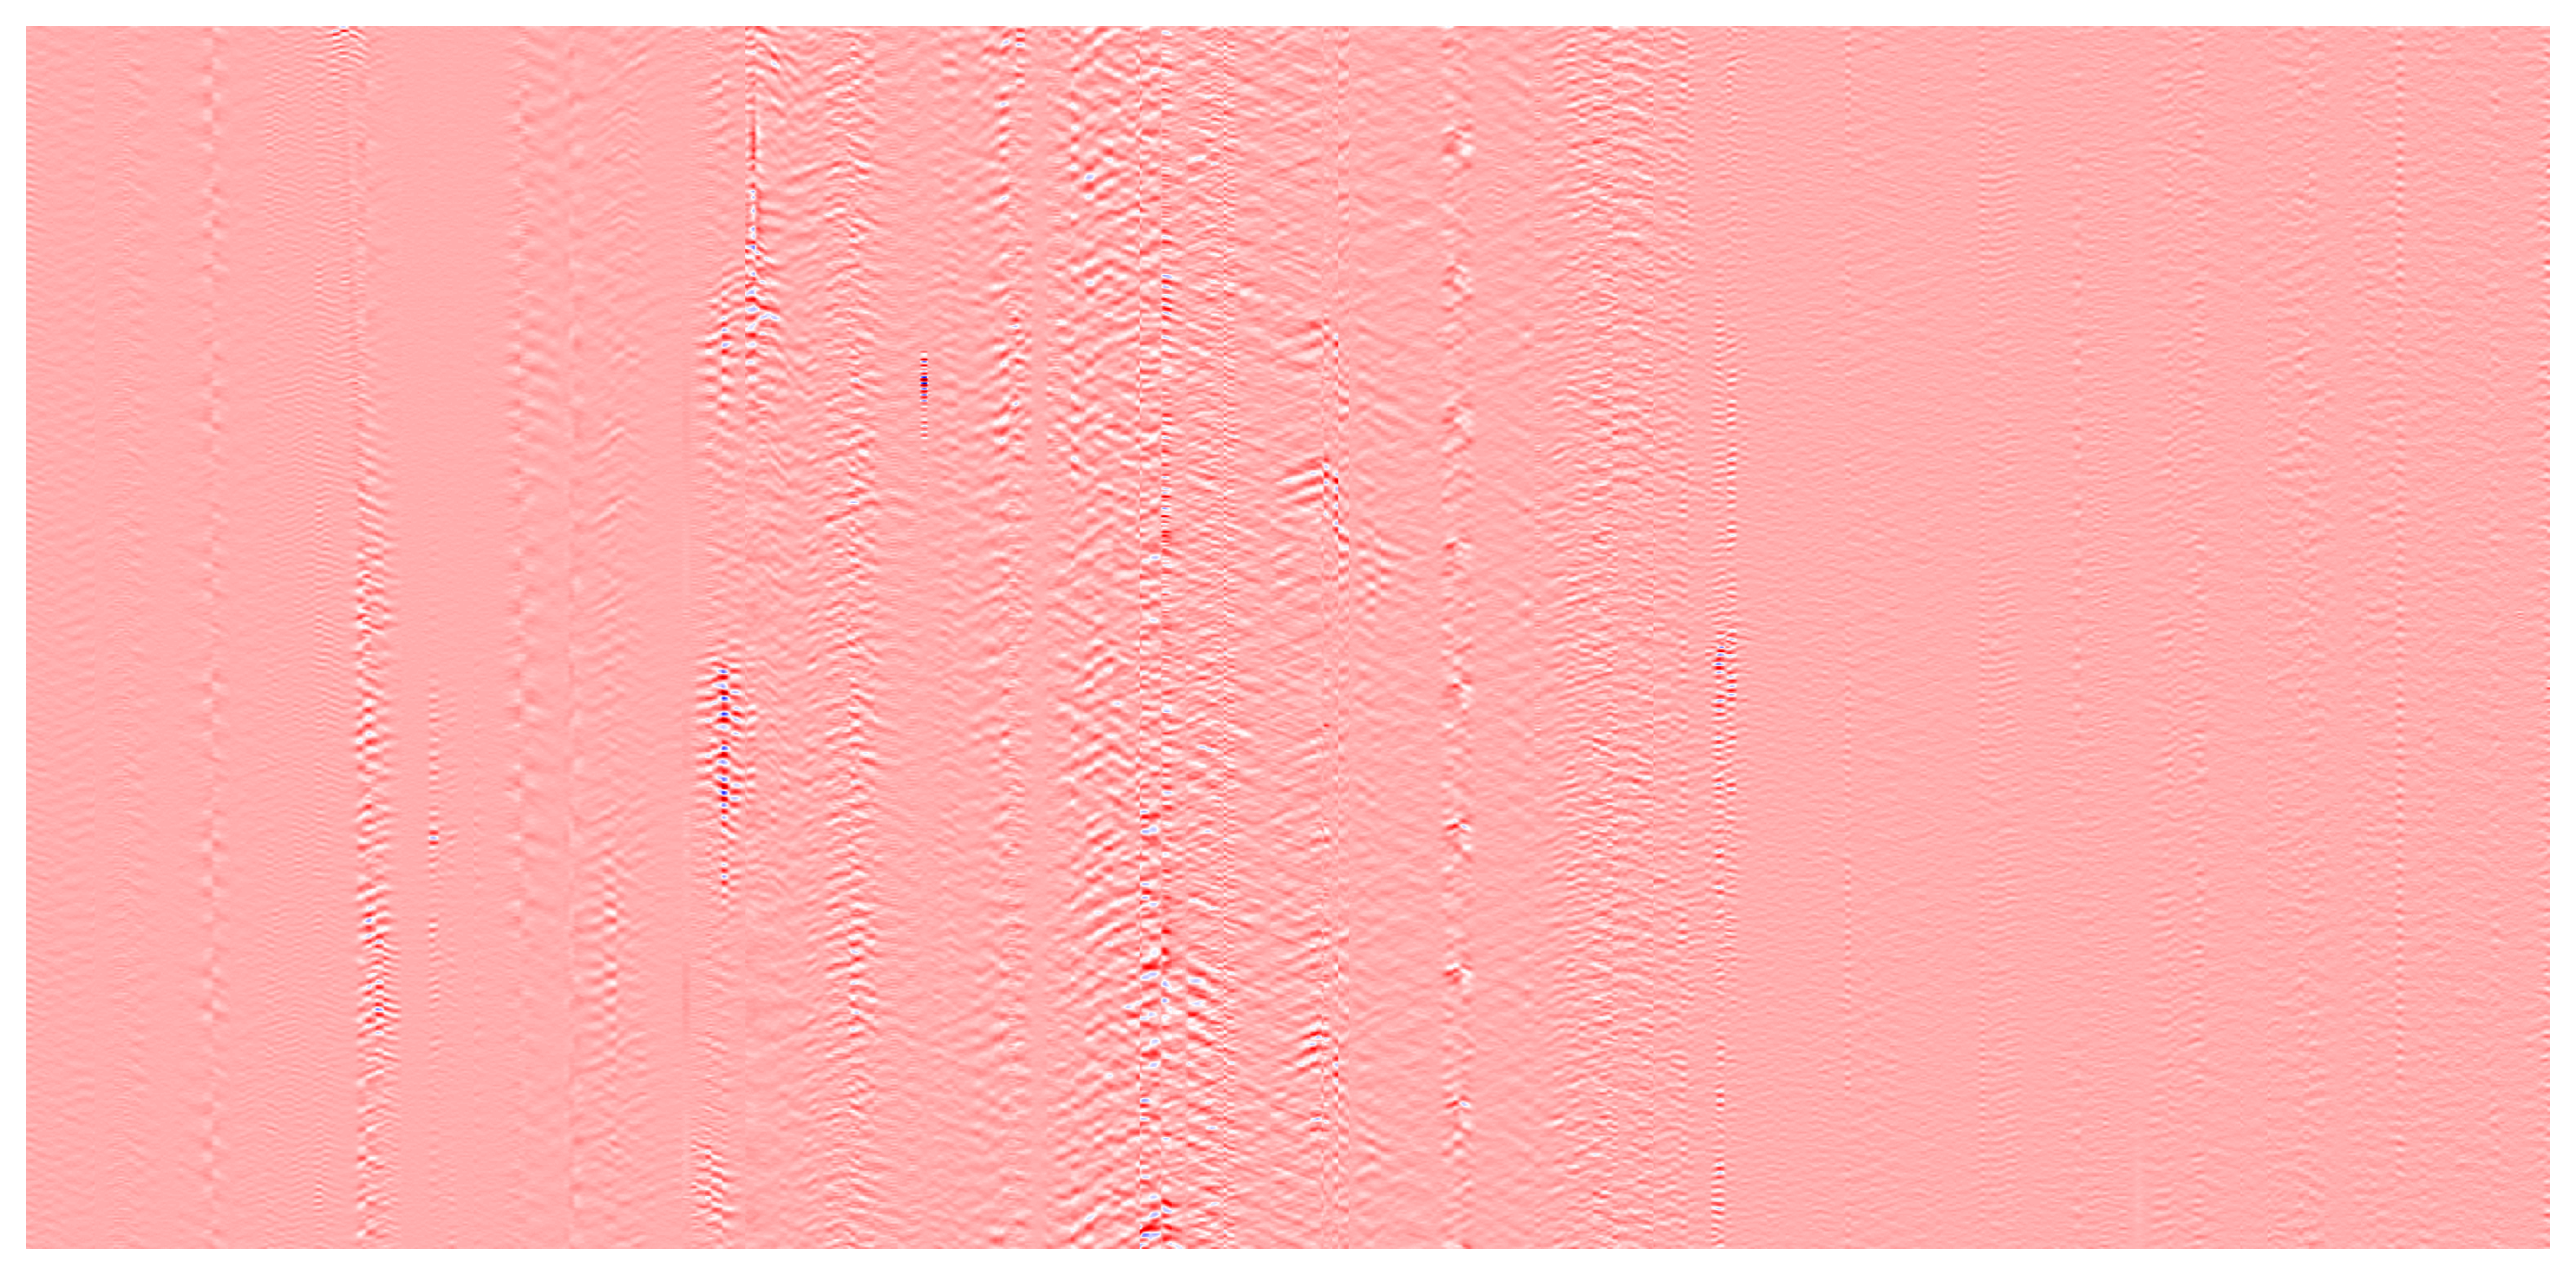
\includegraphics[width=\textwidth]{figures/anomalies/before/20190415_031755.png}
    \end{subfigure}
    
    \vspace{1em}
    
    % Row 2 (Model 1)
    \begin{subfigure}{0.33\textwidth}
        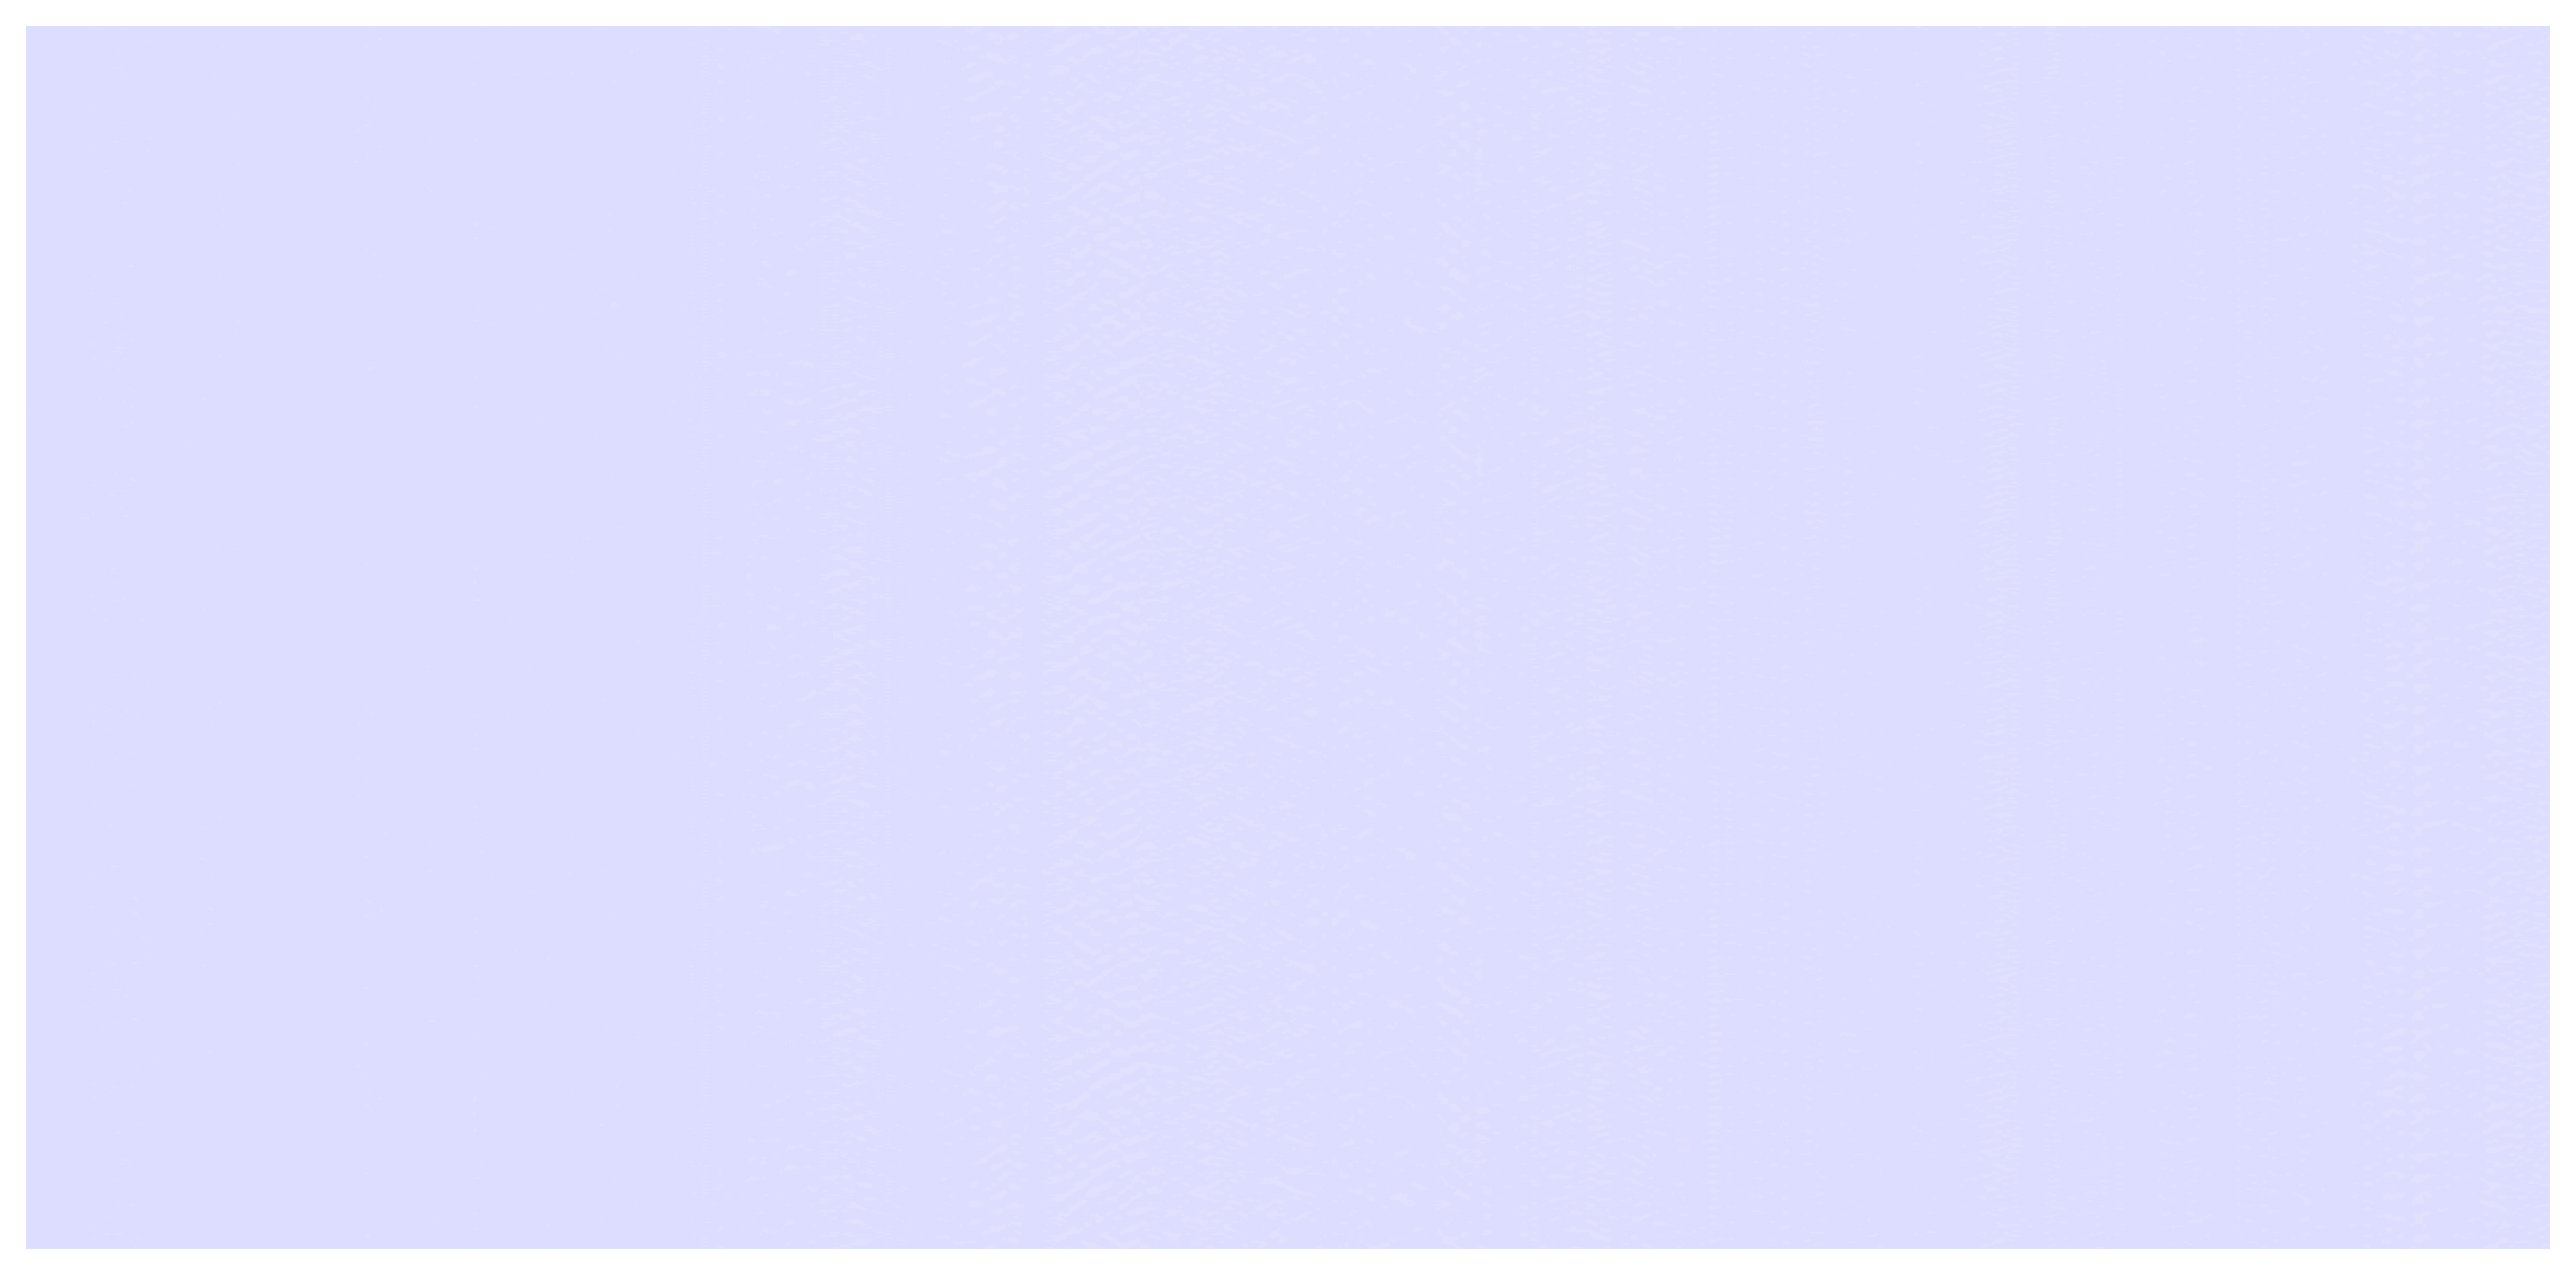
\includegraphics[width=\textwidth]{figures/anomalies/ae/20190415_031735.png}
    \end{subfigure}%
    \hfill
    \begin{subfigure}{0.33\textwidth}
        
\includegraphics[width=\textwidth]{figures/anomalies/ae/20190415_031750.png}
    \end{subfigure}%
    \hfill
    \begin{subfigure}{0.33\textwidth}
        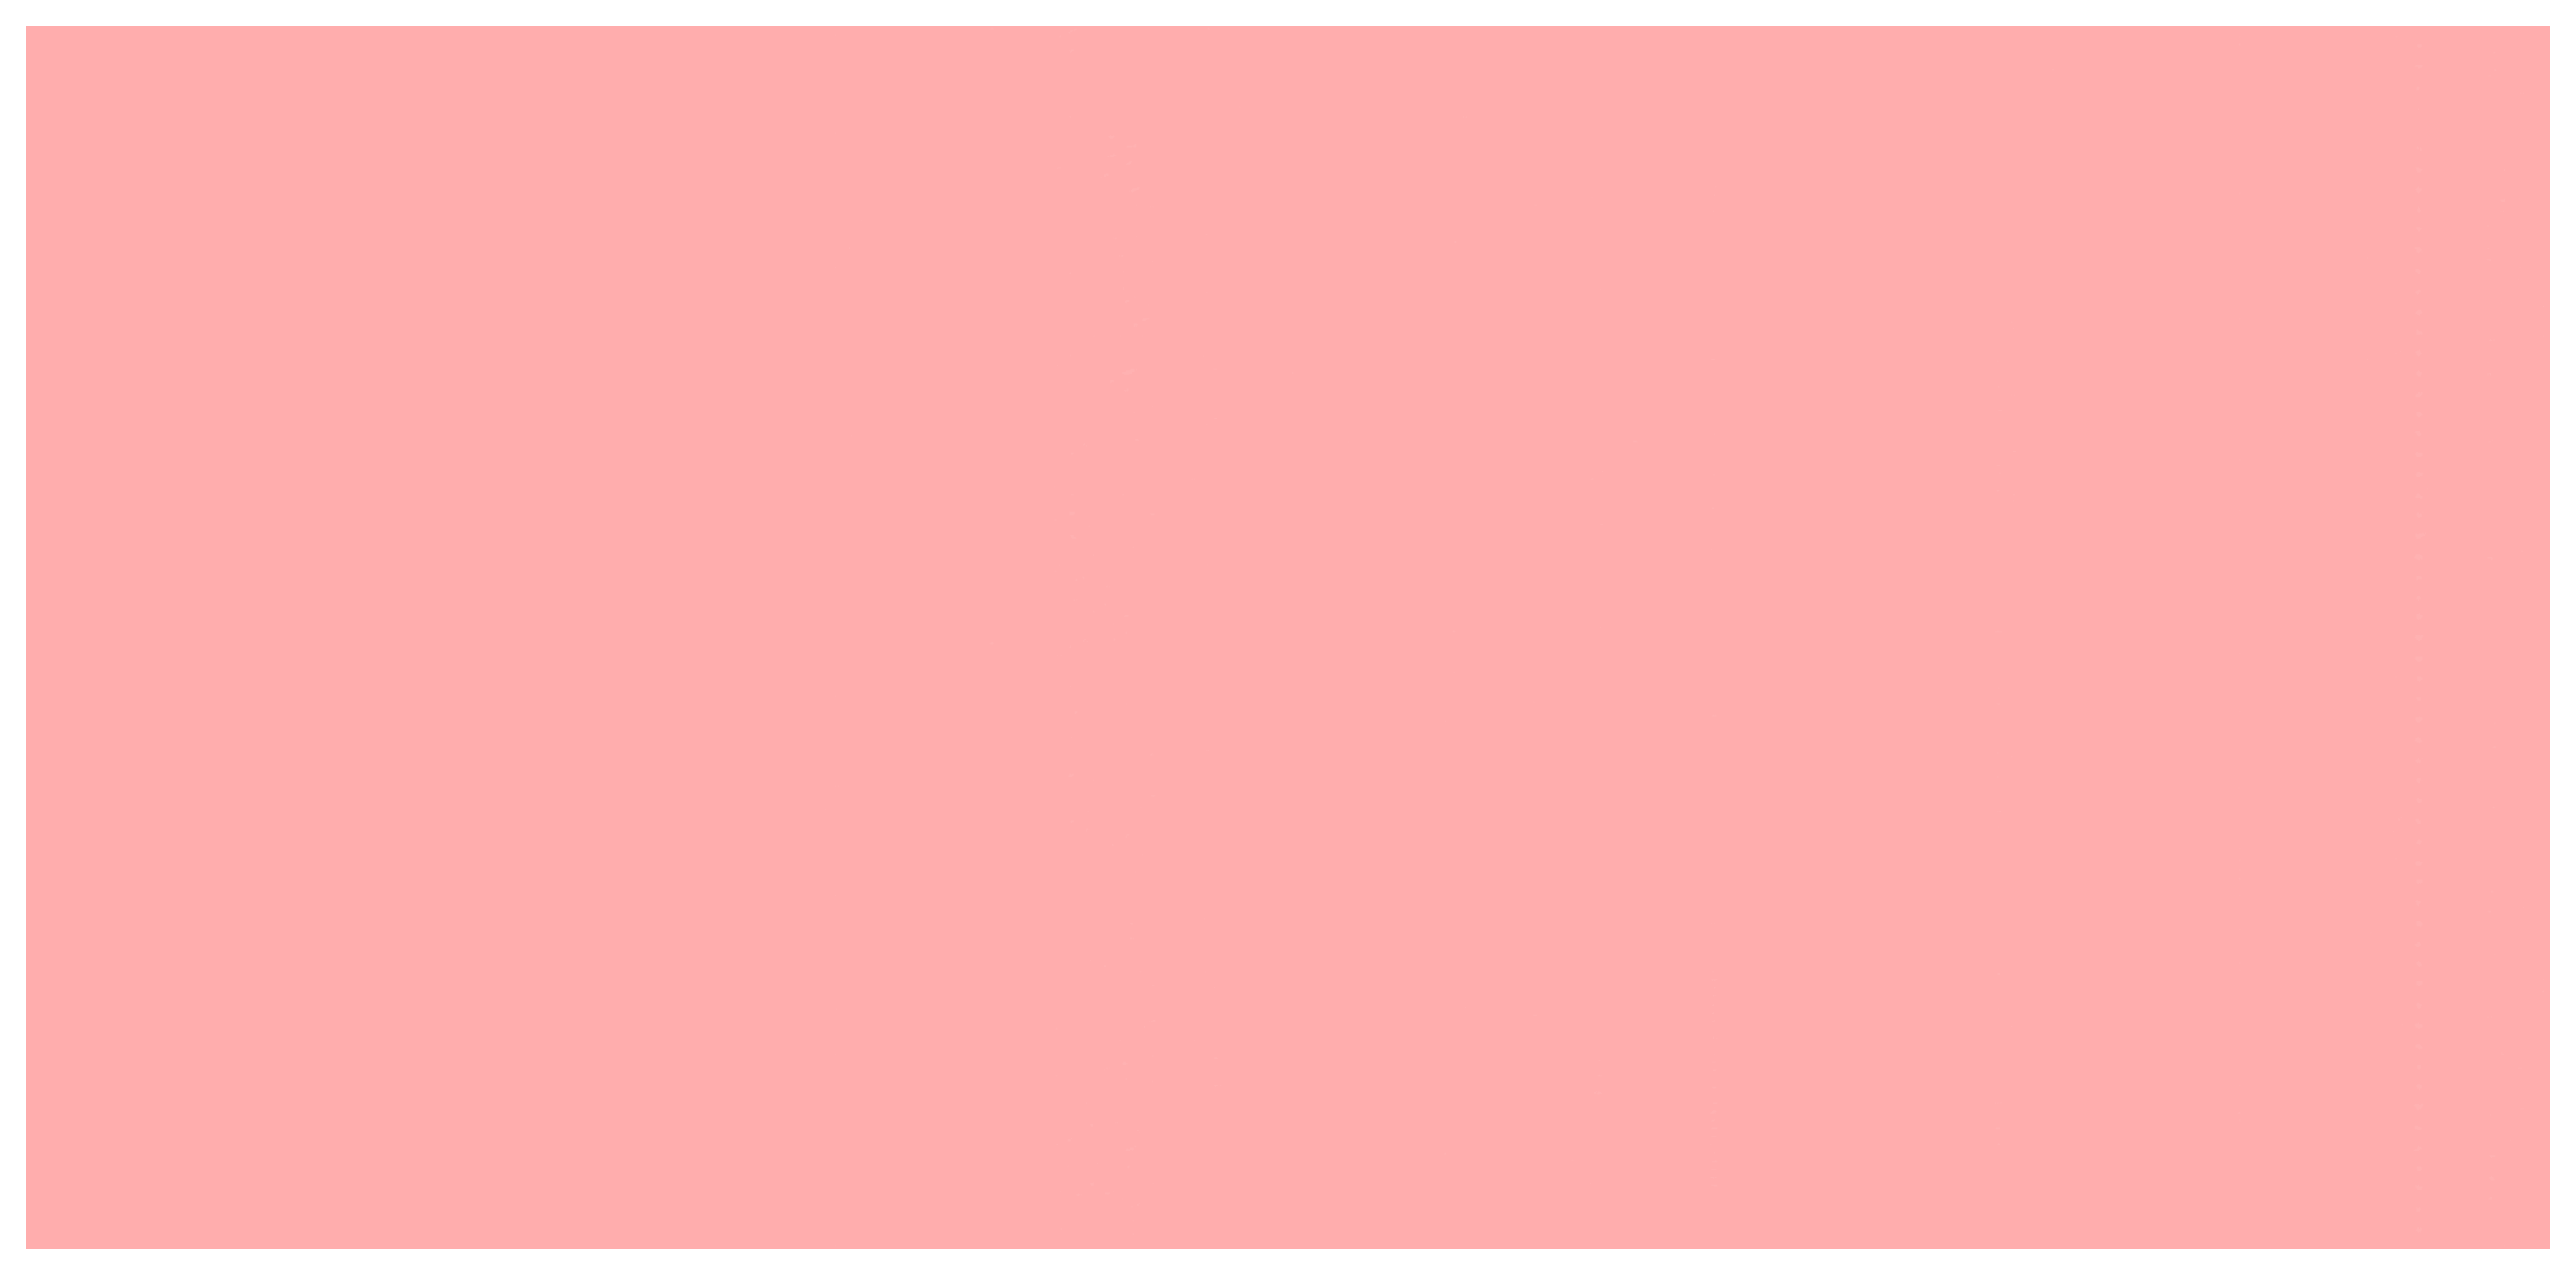
\includegraphics[width=\textwidth]{figures/anomalies/ae/20190415_031755.png}
    \end{subfigure}
    
    \vspace{1em}
    
    
    % Row 4 (Model 3)
    \begin{subfigure}{0.33\textwidth}
        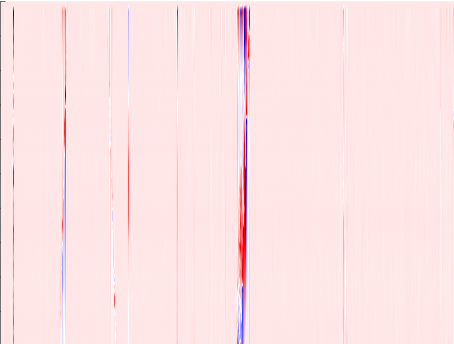
\includegraphics[width=\textwidth]{figures/test.png}
    \end{subfigure}%
    \hfill
    \begin{subfigure}{0.33\textwidth}
        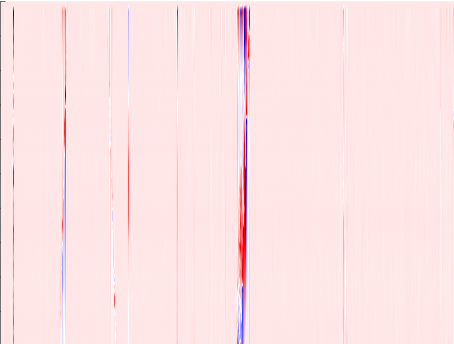
\includegraphics[width=\textwidth]{figures/test.png}
    \end{subfigure}%
    \hfill
    \begin{subfigure}{0.33\textwidth}
        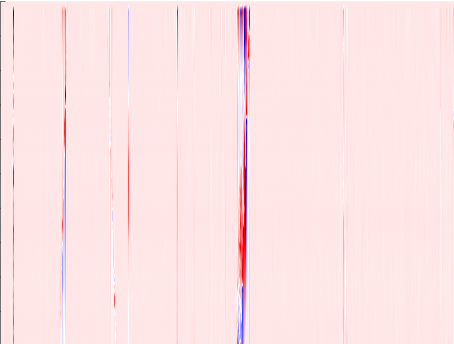
\includegraphics[width=\textwidth]{figures/test.png}
    \end{subfigure}


    \vspace{1em}
    
    % Row 3 (Model 2)
    \begin{subfigure}{0.33\textwidth}
        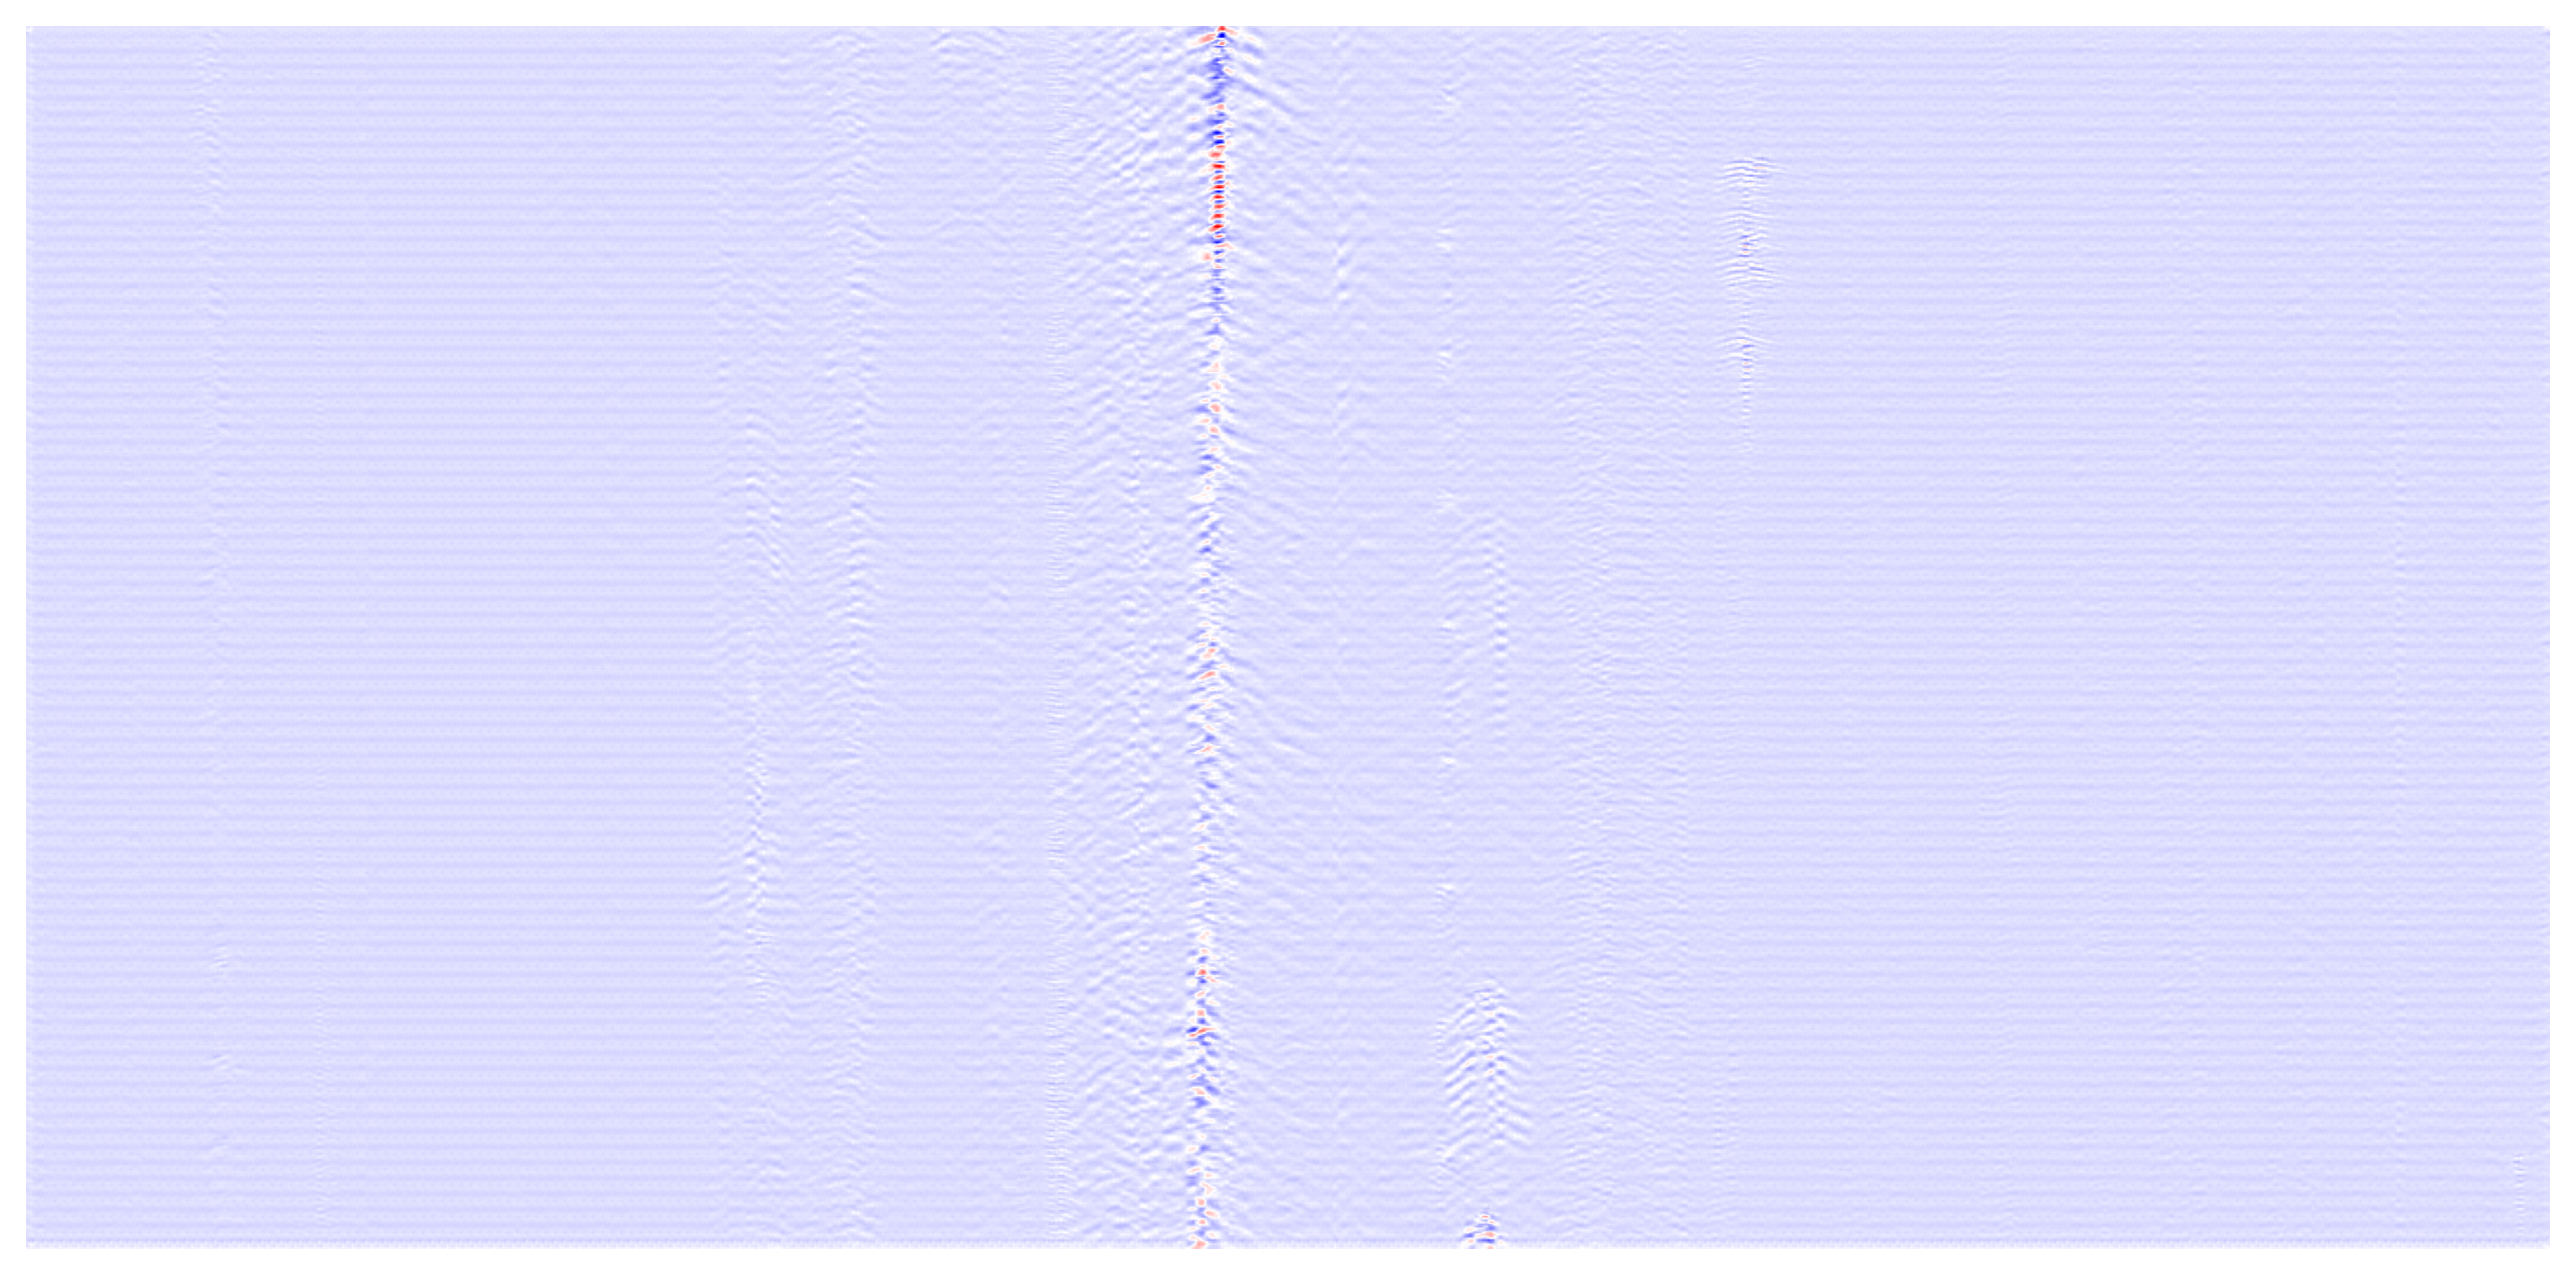
\includegraphics[width=\textwidth]{figures/anomalies/cae/20190415_031735.png}
    \end{subfigure}%
    \hfill
    \begin{subfigure}{0.33\textwidth}
        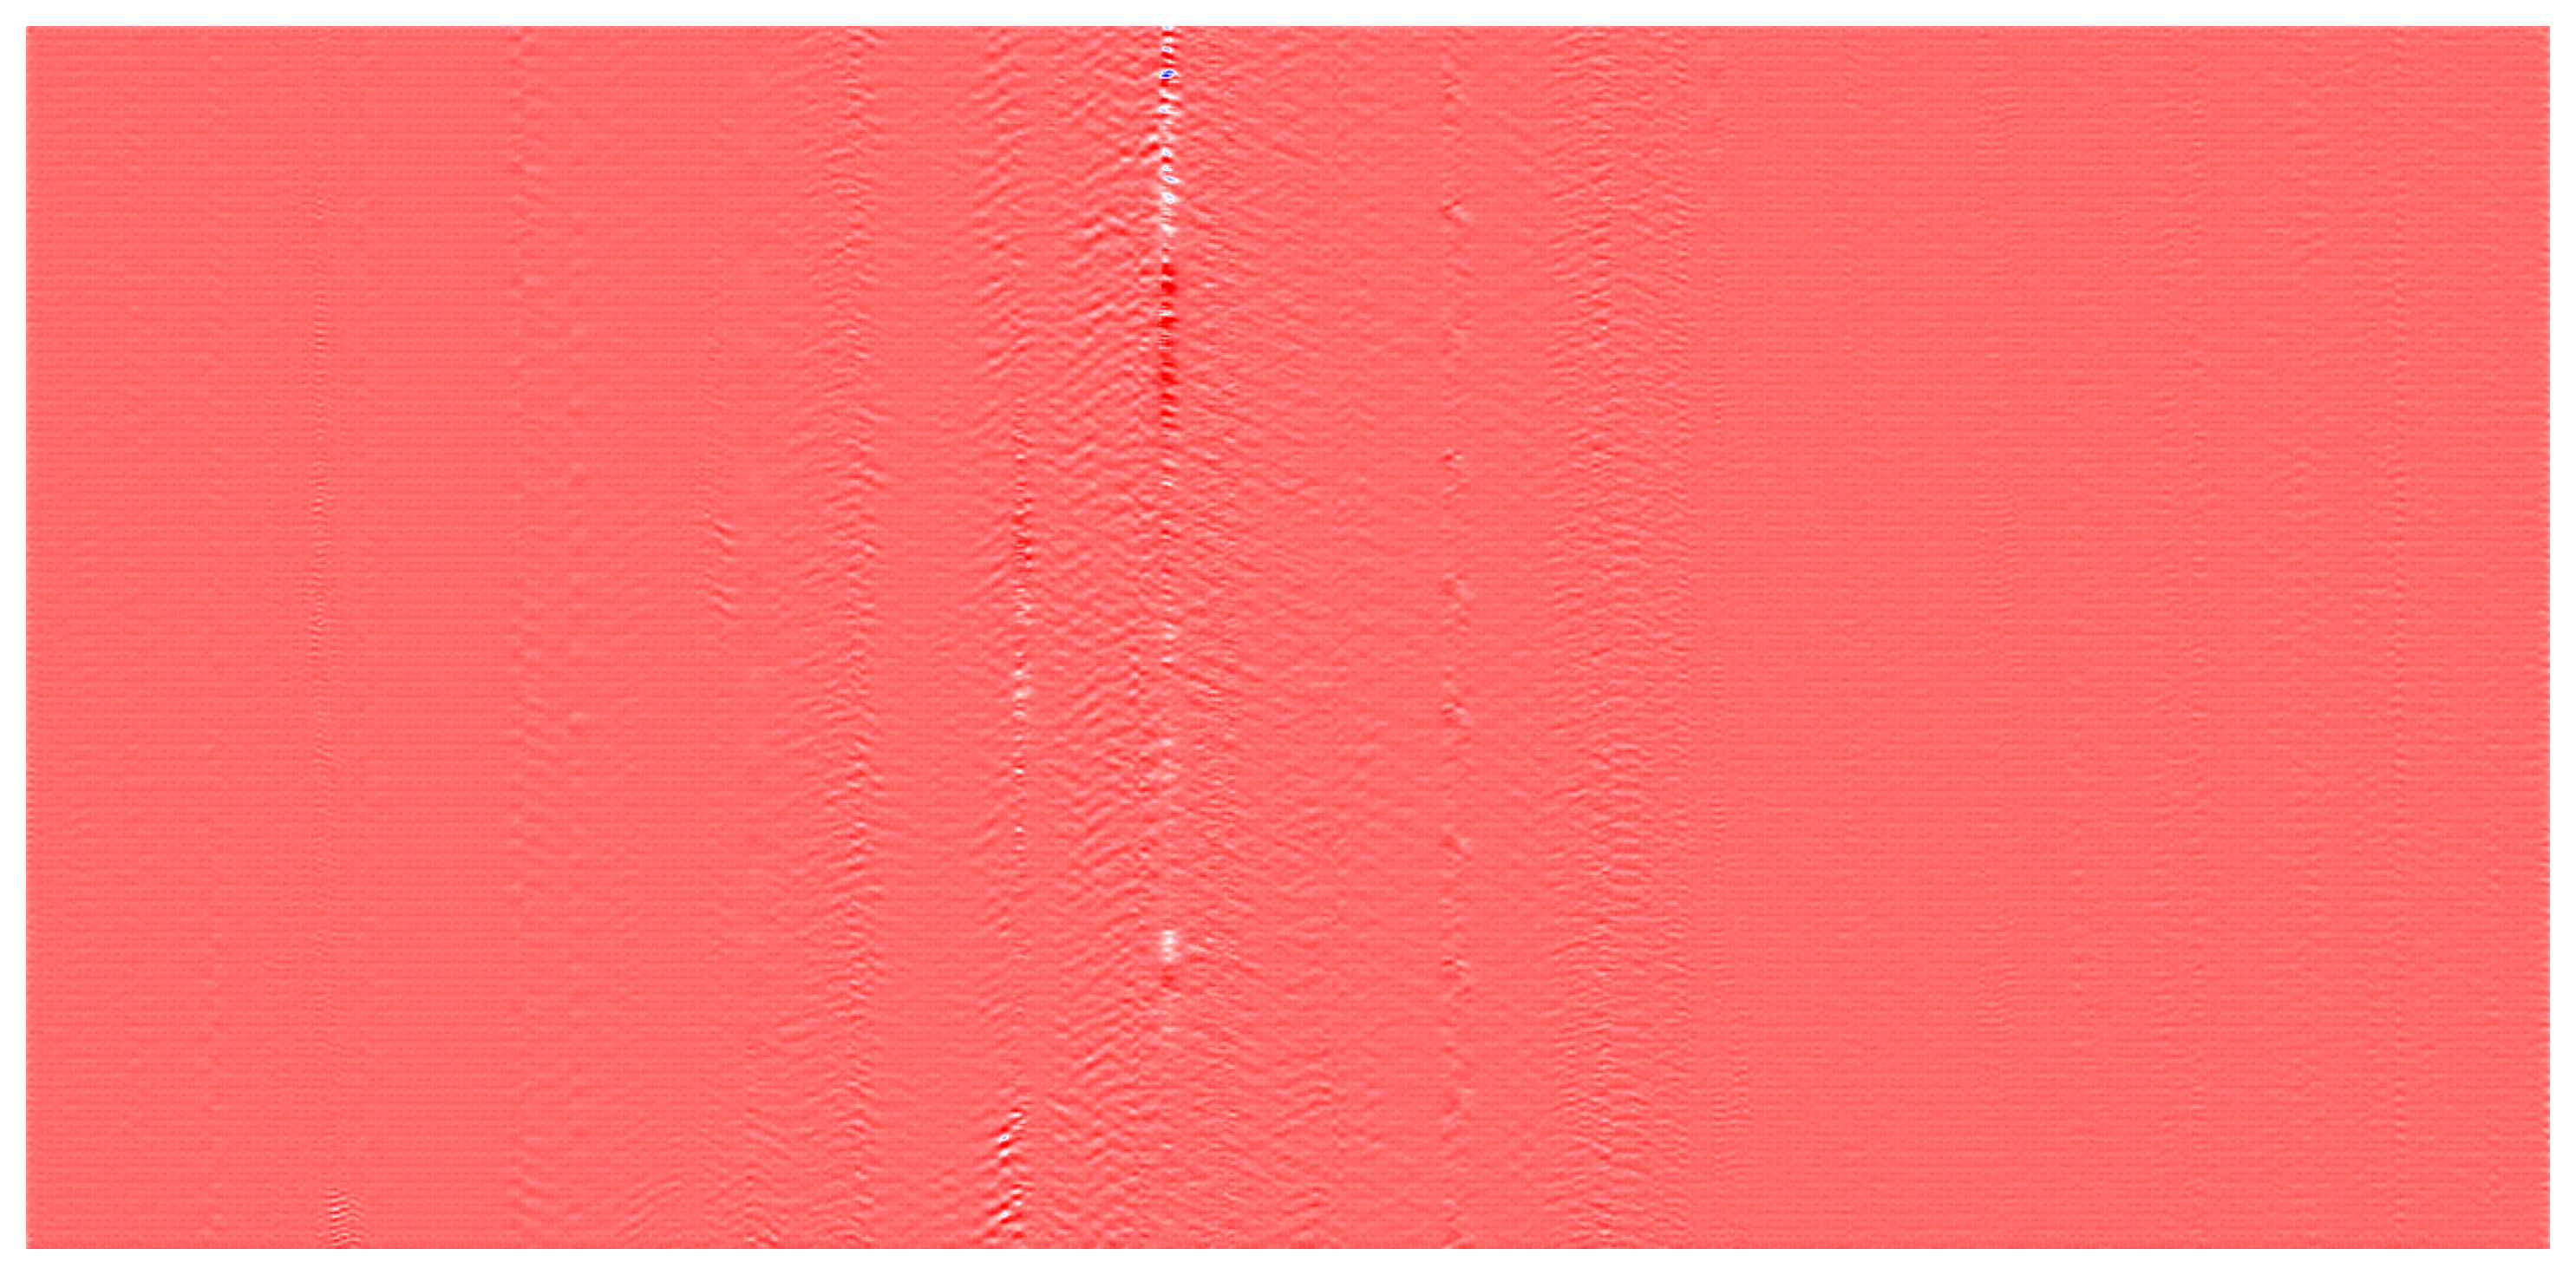
\includegraphics[width=\textwidth]{figures/anomalies/cae/20190415_031750.png}
    \end{subfigure}%
    \hfill
    \begin{subfigure}{0.33\textwidth}
        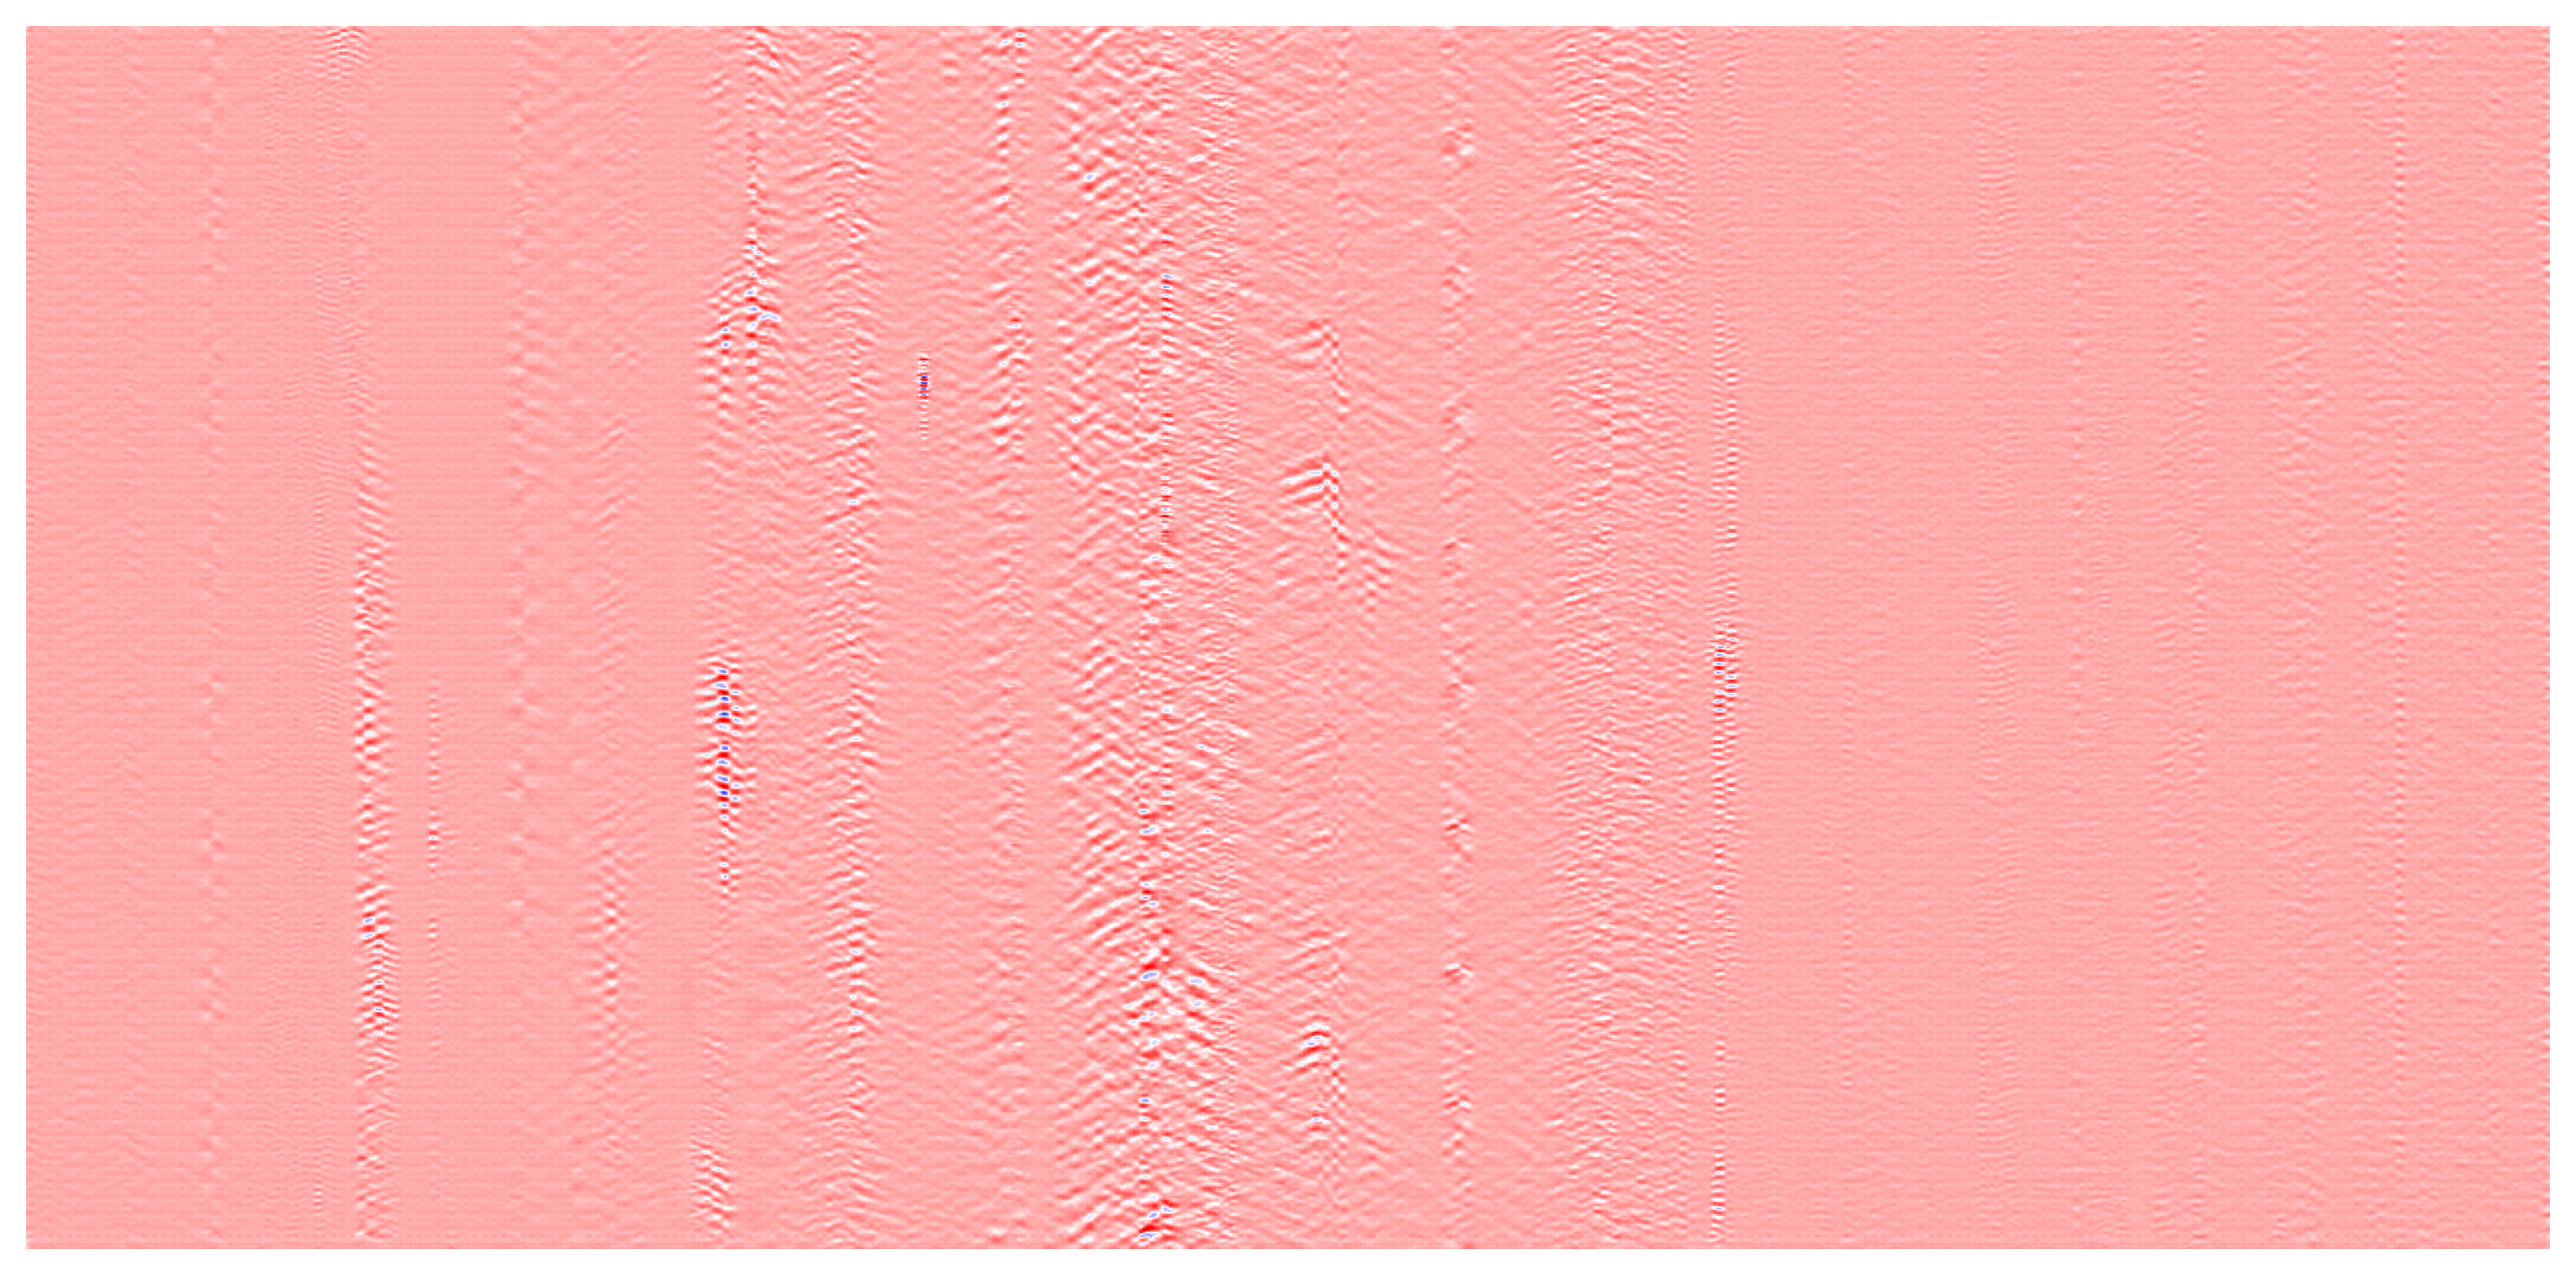
\includegraphics[width=\textwidth]{figures/anomalies/cae/20190415_031755.png}
    \end{subfigure}
    
    
    \vspace{1em}
    
    % Row 5 (Model 4)
    \begin{subfigure}{0.33\textwidth}
        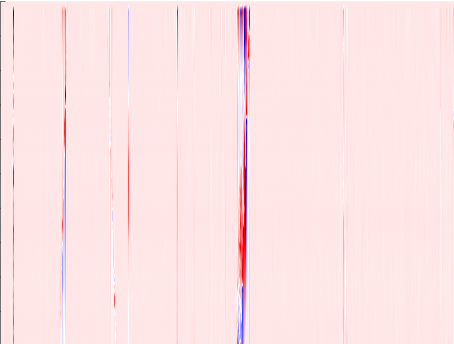
\includegraphics[width=\textwidth]{figures/test.png}
    \end{subfigure}%
    \hfill
    \begin{subfigure}{0.33\textwidth}
        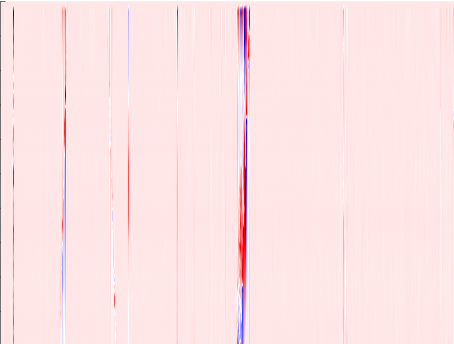
\includegraphics[width=\textwidth]{figures/test.png}
    \end{subfigure}%
    \hfill
    \begin{subfigure}{0.33\textwidth}
        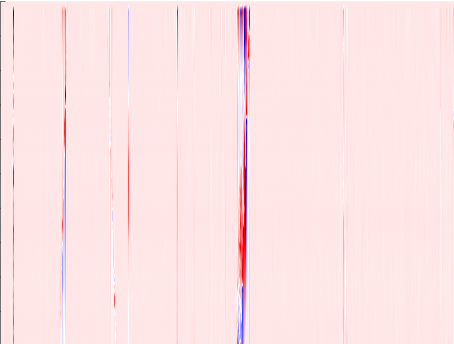
\includegraphics[width=\textwidth]{figures/test.png}
    \end{subfigure}
    
    \caption{Comparison of original images and their reconstructions by different autoencoders. The top row is the original \acrshort{das} heatmap, followed by: AE, $\beta$-VAE, CAE and $\beta$-CVAE}
    \label{fig:aereconstruct}
\end{figure}

\subsection{Experiment \rnum{2}: Anomaly Detection}

An important part of analyzing our autoencoders is the choice of metrics. Whereas loss and accuracy can provide proficient details about the model training itself, other metrics are better suited for analyzing the 

Table \ref{tab:autoencoder_comparison} presents a comparative analysis of the four autoencoder types: dense, convolutional, variational dense, and variational convolutional.





\begin{table}[!htbp]
\centering
\label{tab:confusion-matrix-results}
\begin{tabular}{l
    S[table-format=3.0]
    S[table-format=3.0]
    S[table-format=3.0]
    S[table-format=3.0]
}
\toprule
\textbf{Model} & {\textbf{TP}} & {\textbf{FP}} & {\textbf{TN}} & {\textbf{FN}} \\
\midrule
\rowcolor{gray!10} AE   & 0 & 42 & 418 & 140 \\
$\beta$-VAE  & 101 & 2 & 458 & 39 \\
\rowcolor{gray!10} CAE  & 75 & 9 & 451 & 65 \\
$\beta$-CVAE & \textbf{103} & \textbf{5} & \textbf{455} & \textbf{37} \\
\bottomrule
\end{tabular}
\caption{Confusion Matrix Components}
\end{table}
\begin{table}[!htbp]
\centering
\label{tab:performance-metrics}
\begin{tabular}{l
    S[table-format=1.3]
    S[table-format=1.3]
    S[table-format=1.3]
    S[table-format=1.3]
    S[table-format=1.3]
}
\toprule
\textbf{Model} & {\textbf{Precision}} & {\textbf{Recall (TPR)}} & {\textbf{F1-Score}} & {\textbf{FPR}} & {\textbf{PR AUC}} \\
\midrule
\rowcolor{gray!10} AE   & 0.000 & 0.000 & 0.000 & 0.091 & 0.157 \\
$\beta$-VAE  & \textbf{0.981} & 0.721 & \textbf{0.831} & \textbf{0.004} & \textbf{0.925} \\
\rowcolor{gray!10} CAE  & 0.893 & 0.536 & 0.670 & 0.020 & 0.736 \\
$\beta$-CVAE & 0.954 & \textbf{0.736} & \textbf{0.831} & 0.011 & 0.924 \\
\bottomrule
\end{tabular}
\caption{Model Performance Metrics Comparison}
\end{table}

\begin{figure}[!h]
    \centering
    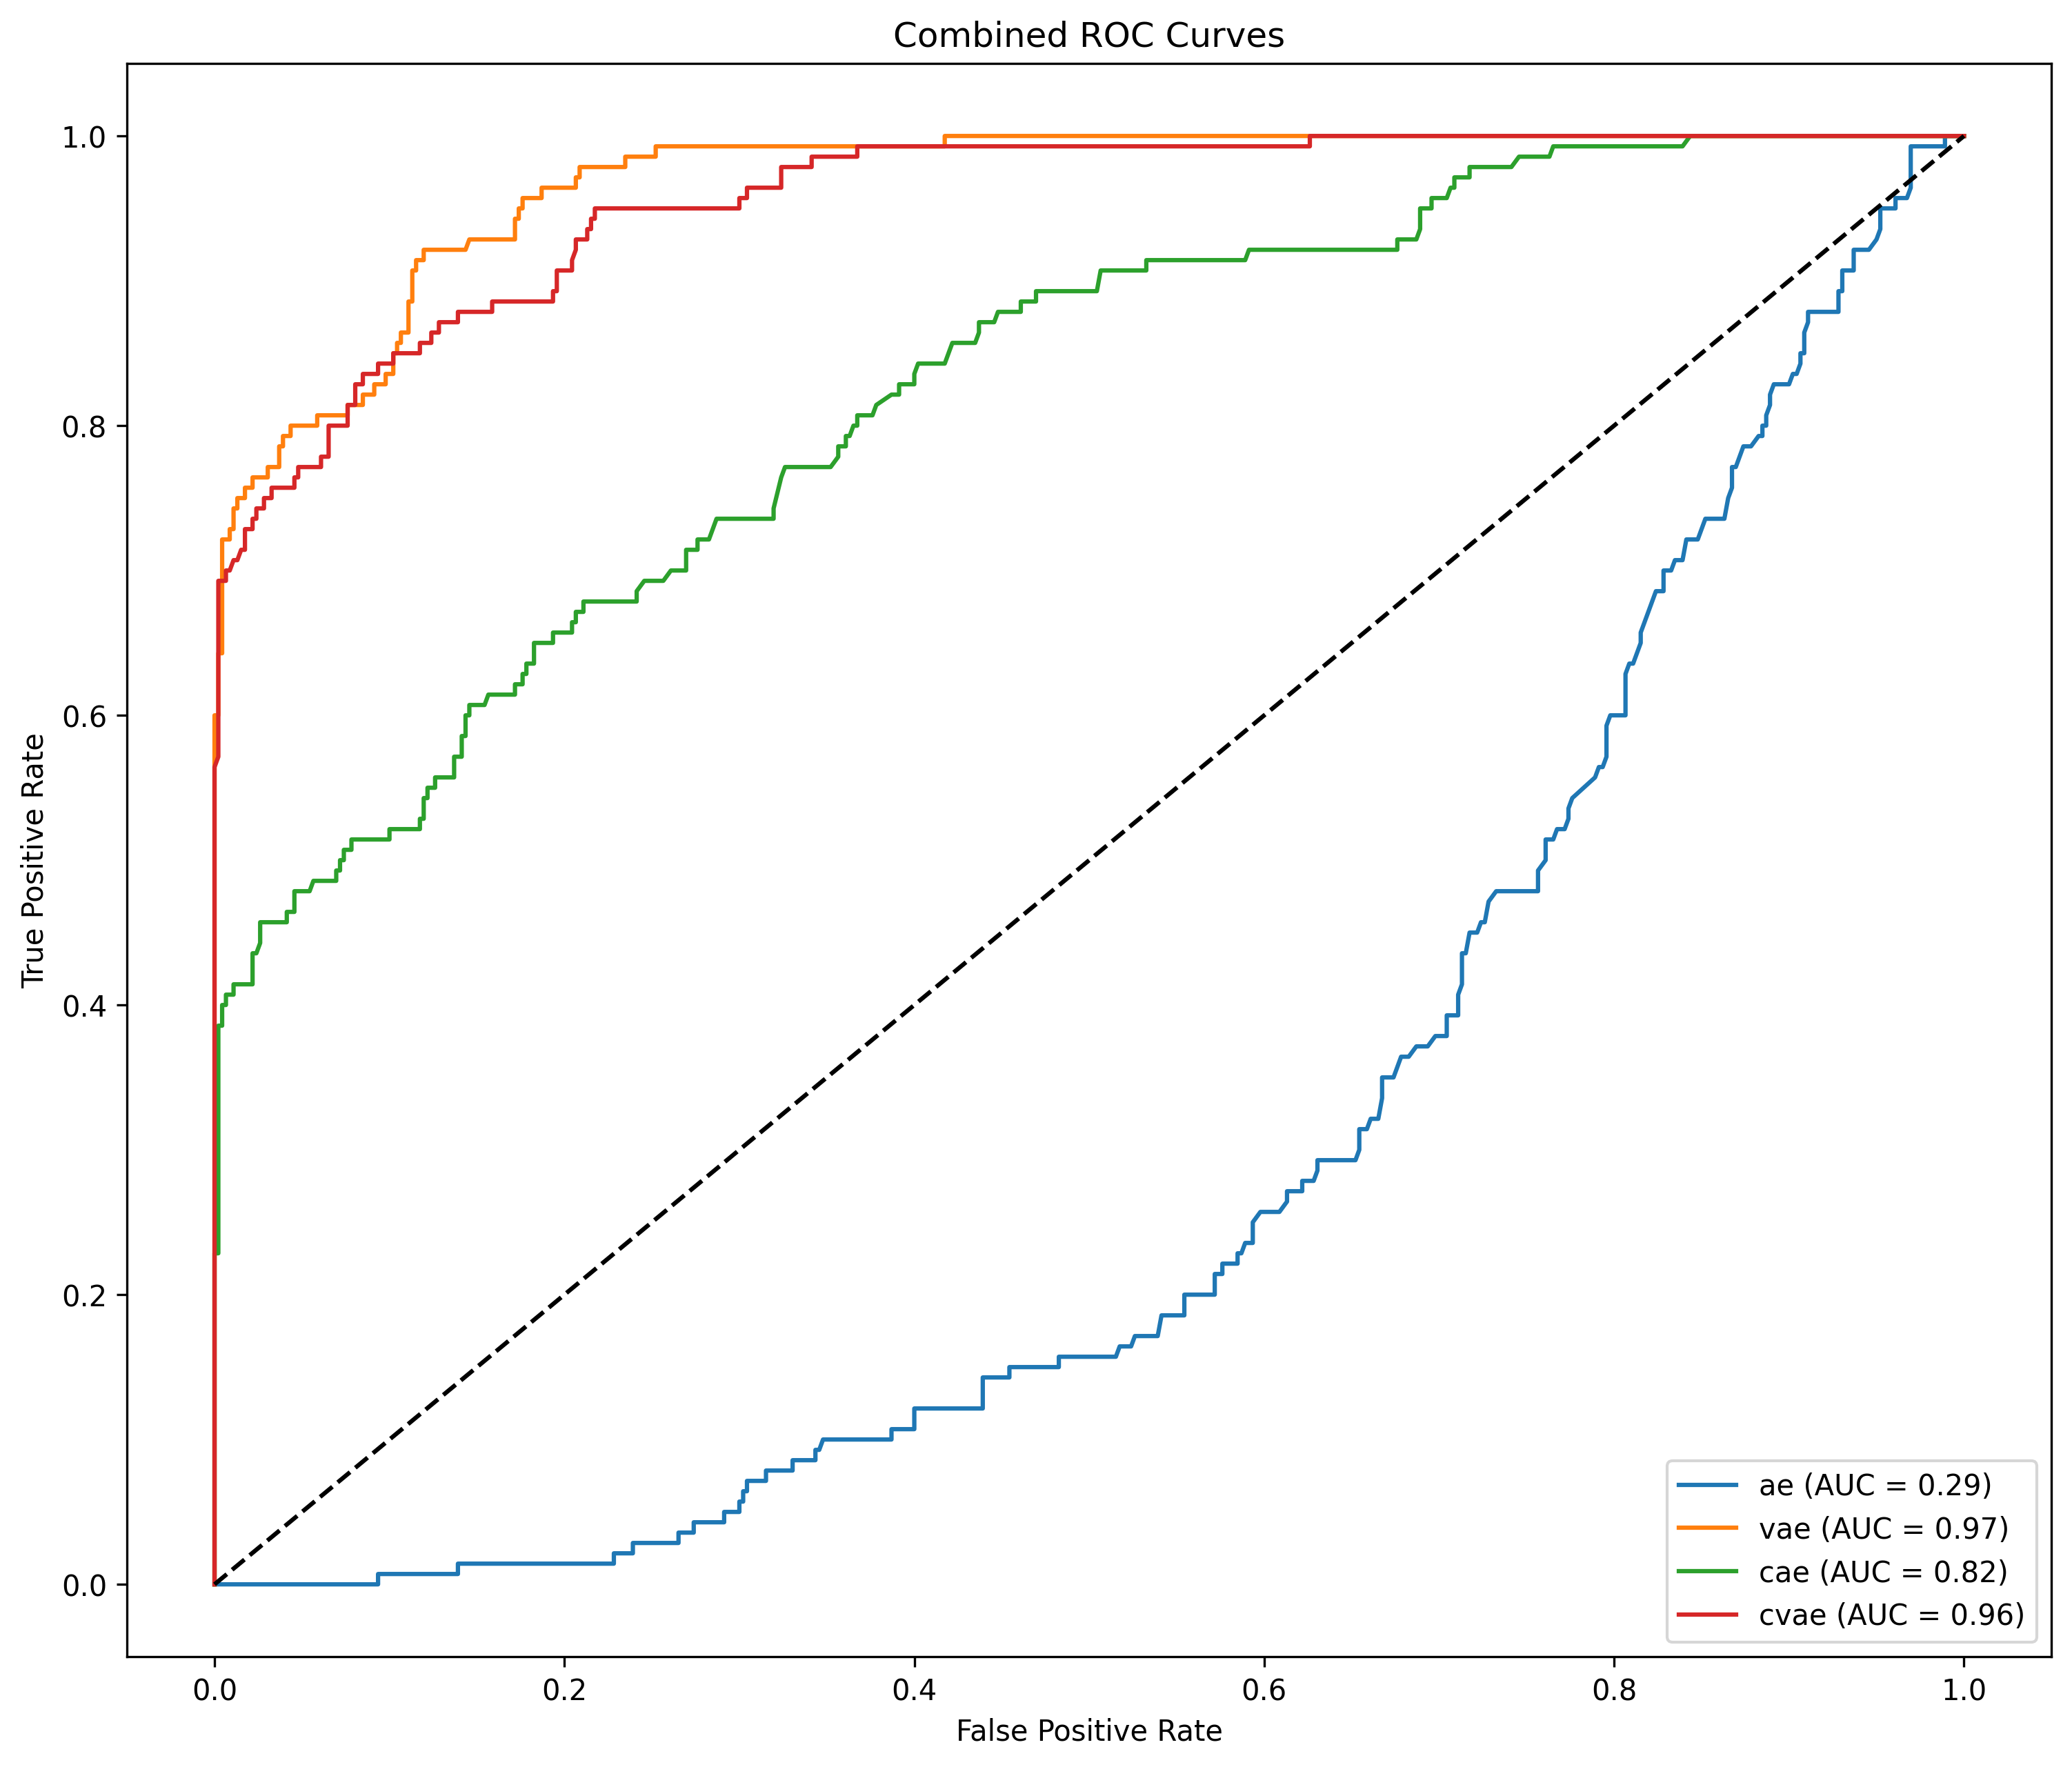
\includegraphics[scale=0.6]{figures/anomalies/combined_roc_curve.png}
    \caption{Combined ROC curve for all models}
    \label{fig:roccurve}
\end{figure}

\begin{figure}[!h]
    \centering
    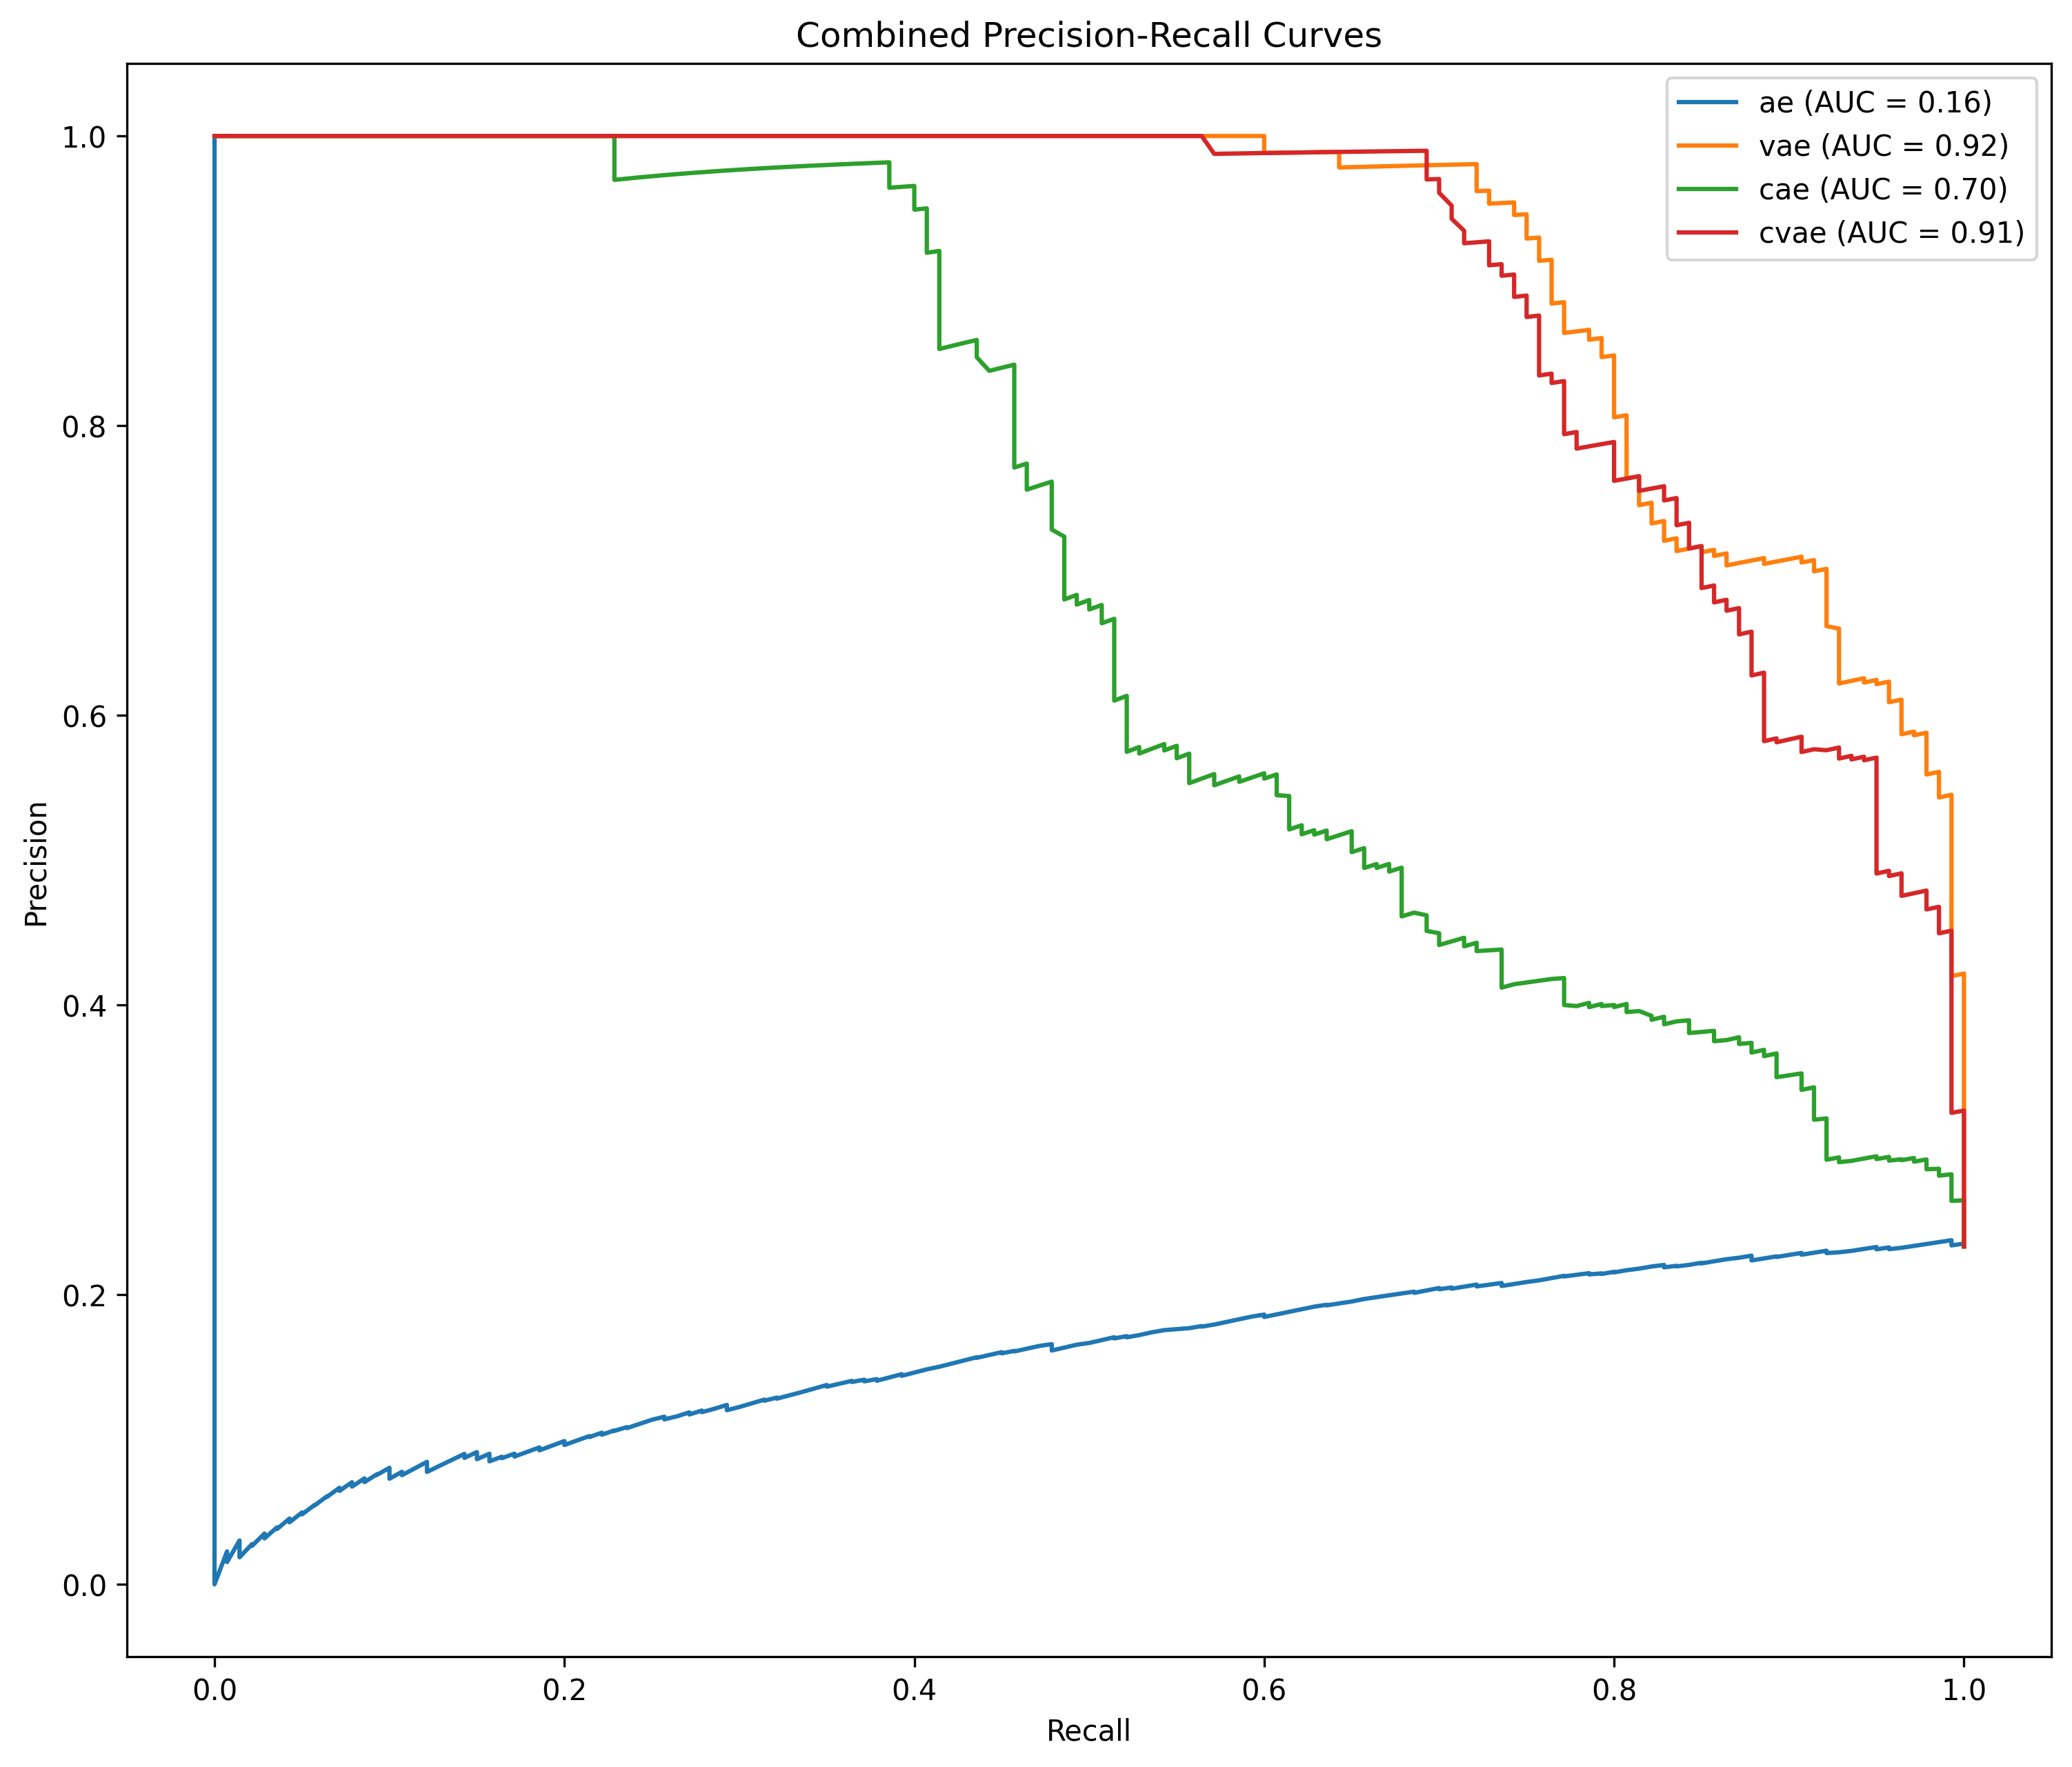
\includegraphics[scale=0.6]{figures/anomalies/combined_pr_curve.png}
    \caption{Combined PR curve for all models}
    \label{fig:prcurve}
\end{figure}



\subsubsection{Threshold Analysis}

\begin{figure}[!h]
  \centering
  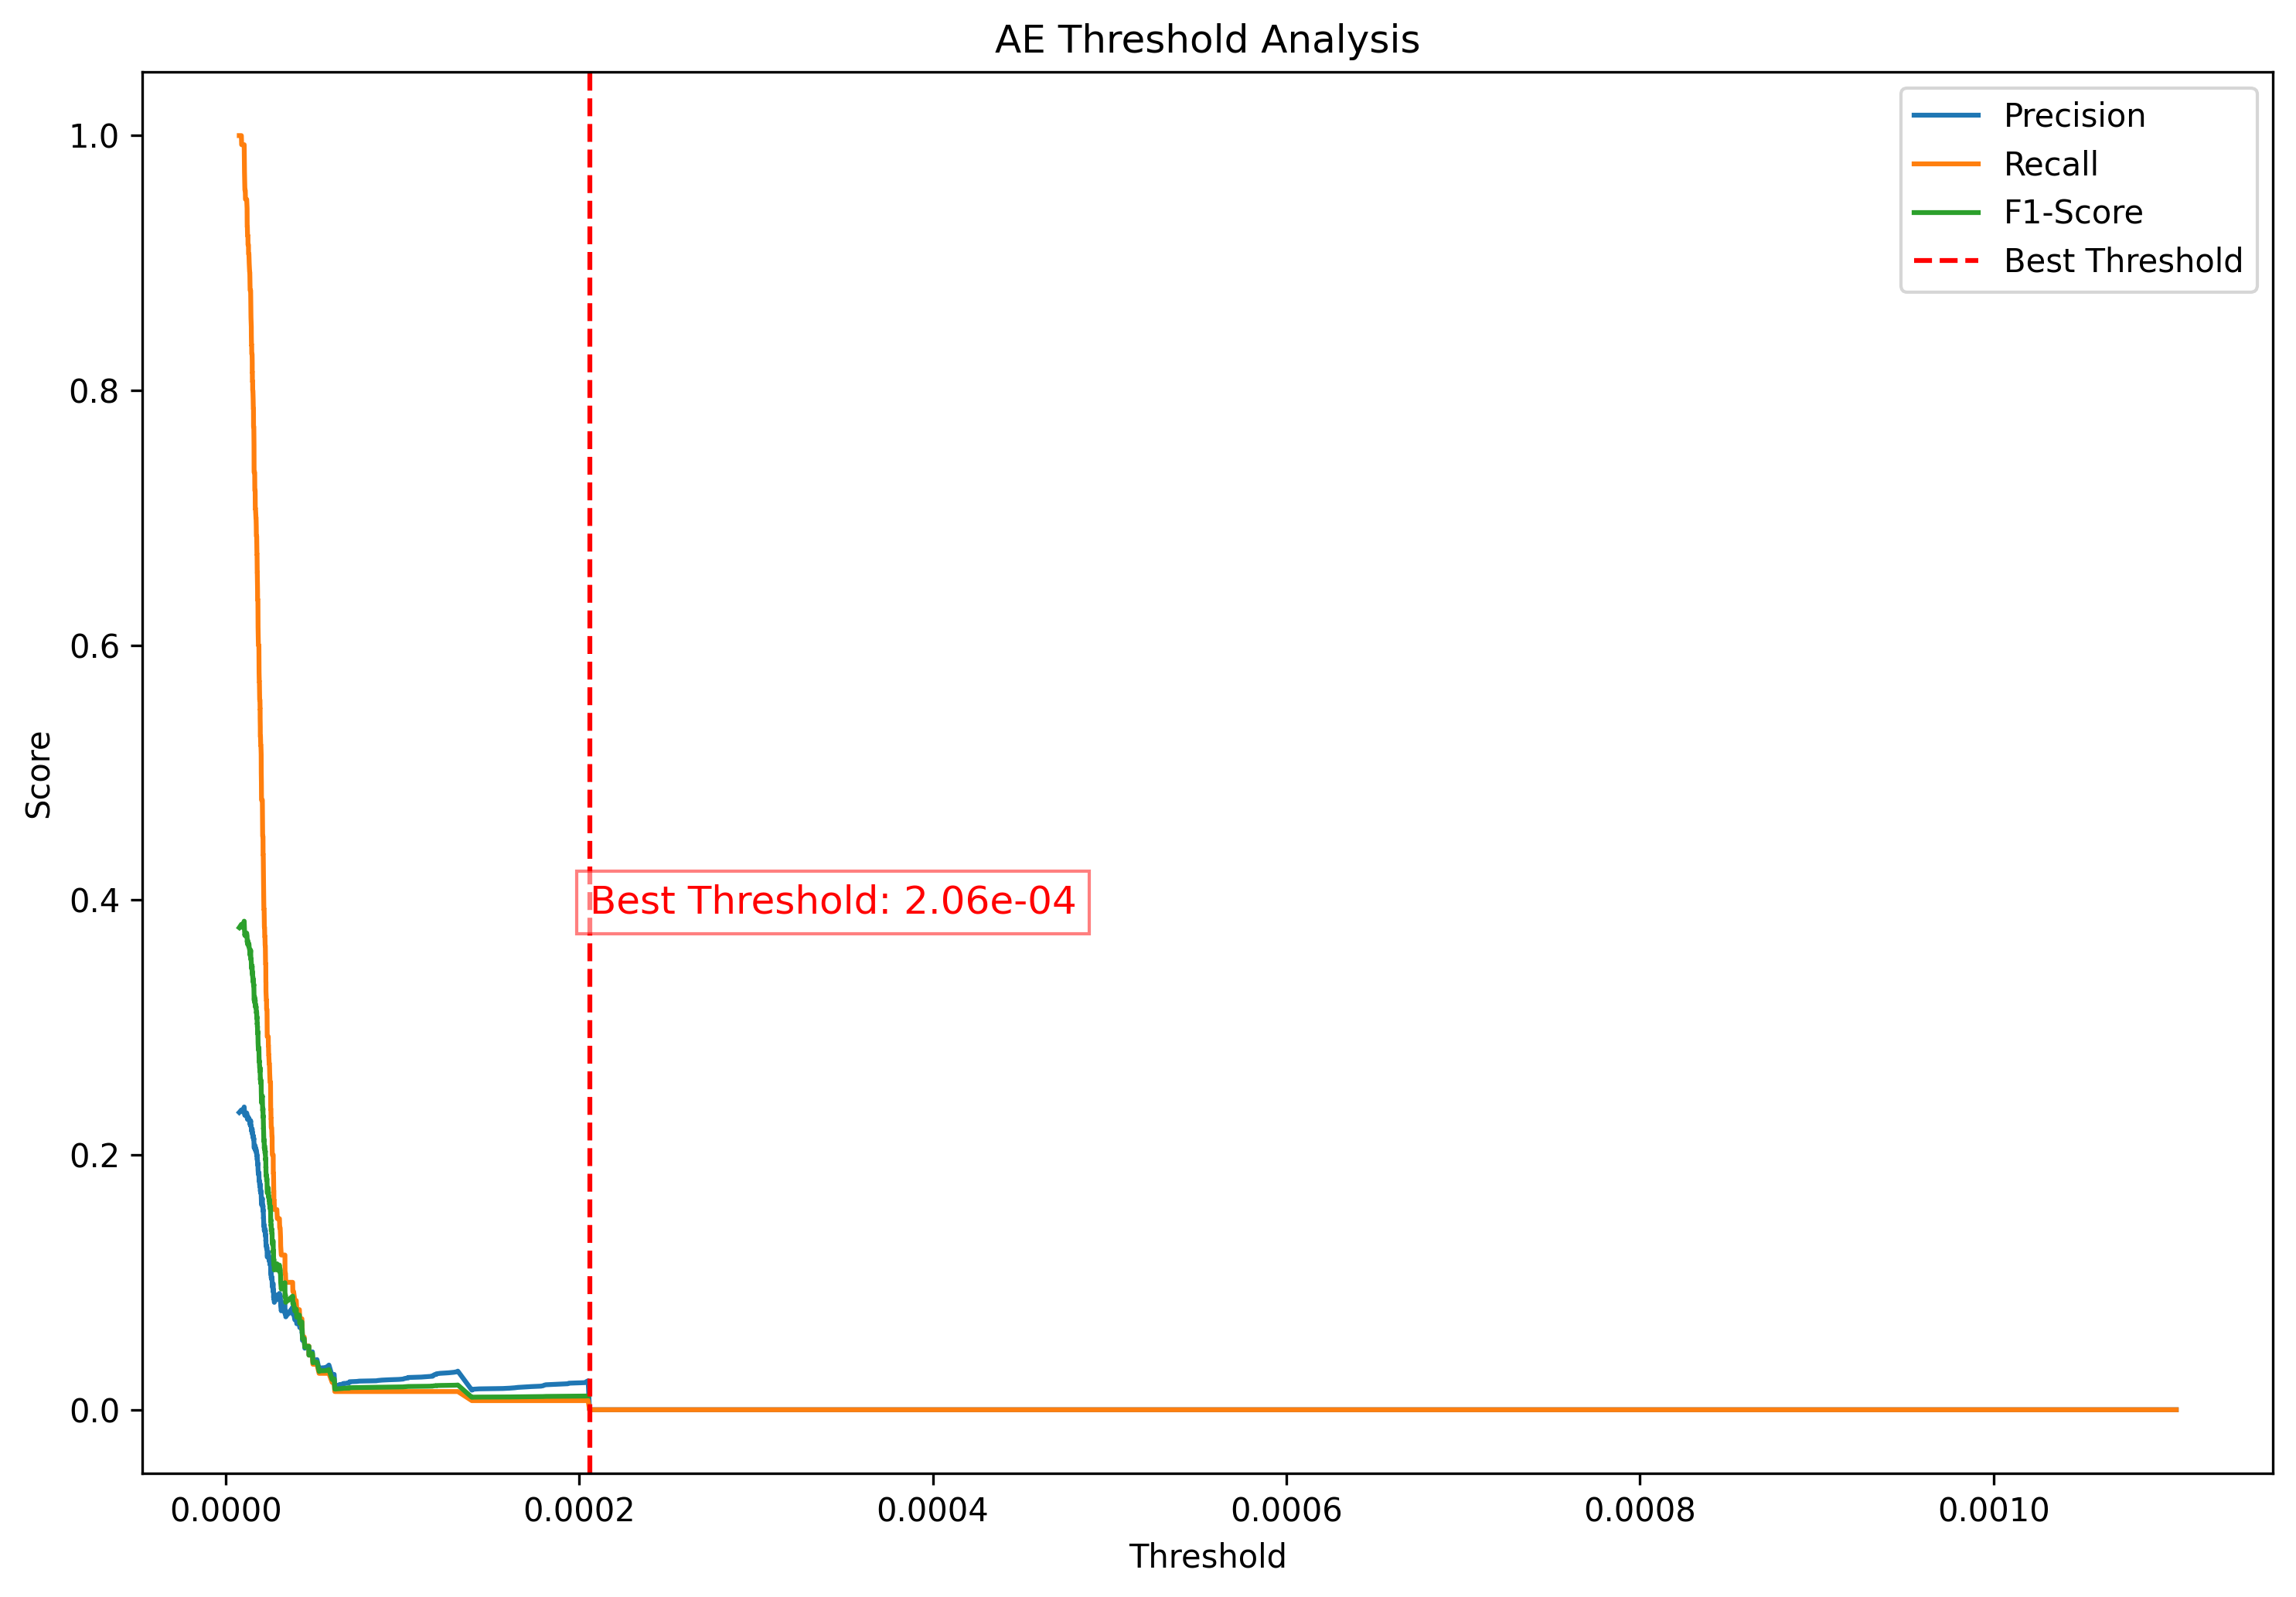
\includegraphics[scale=0.5]{figures/anomalies/ae/threshold.png}
  \caption{AE}
  \label{fig:threshold_ae}
\end{figure}

\begin{figure}[!h]
  \centering
  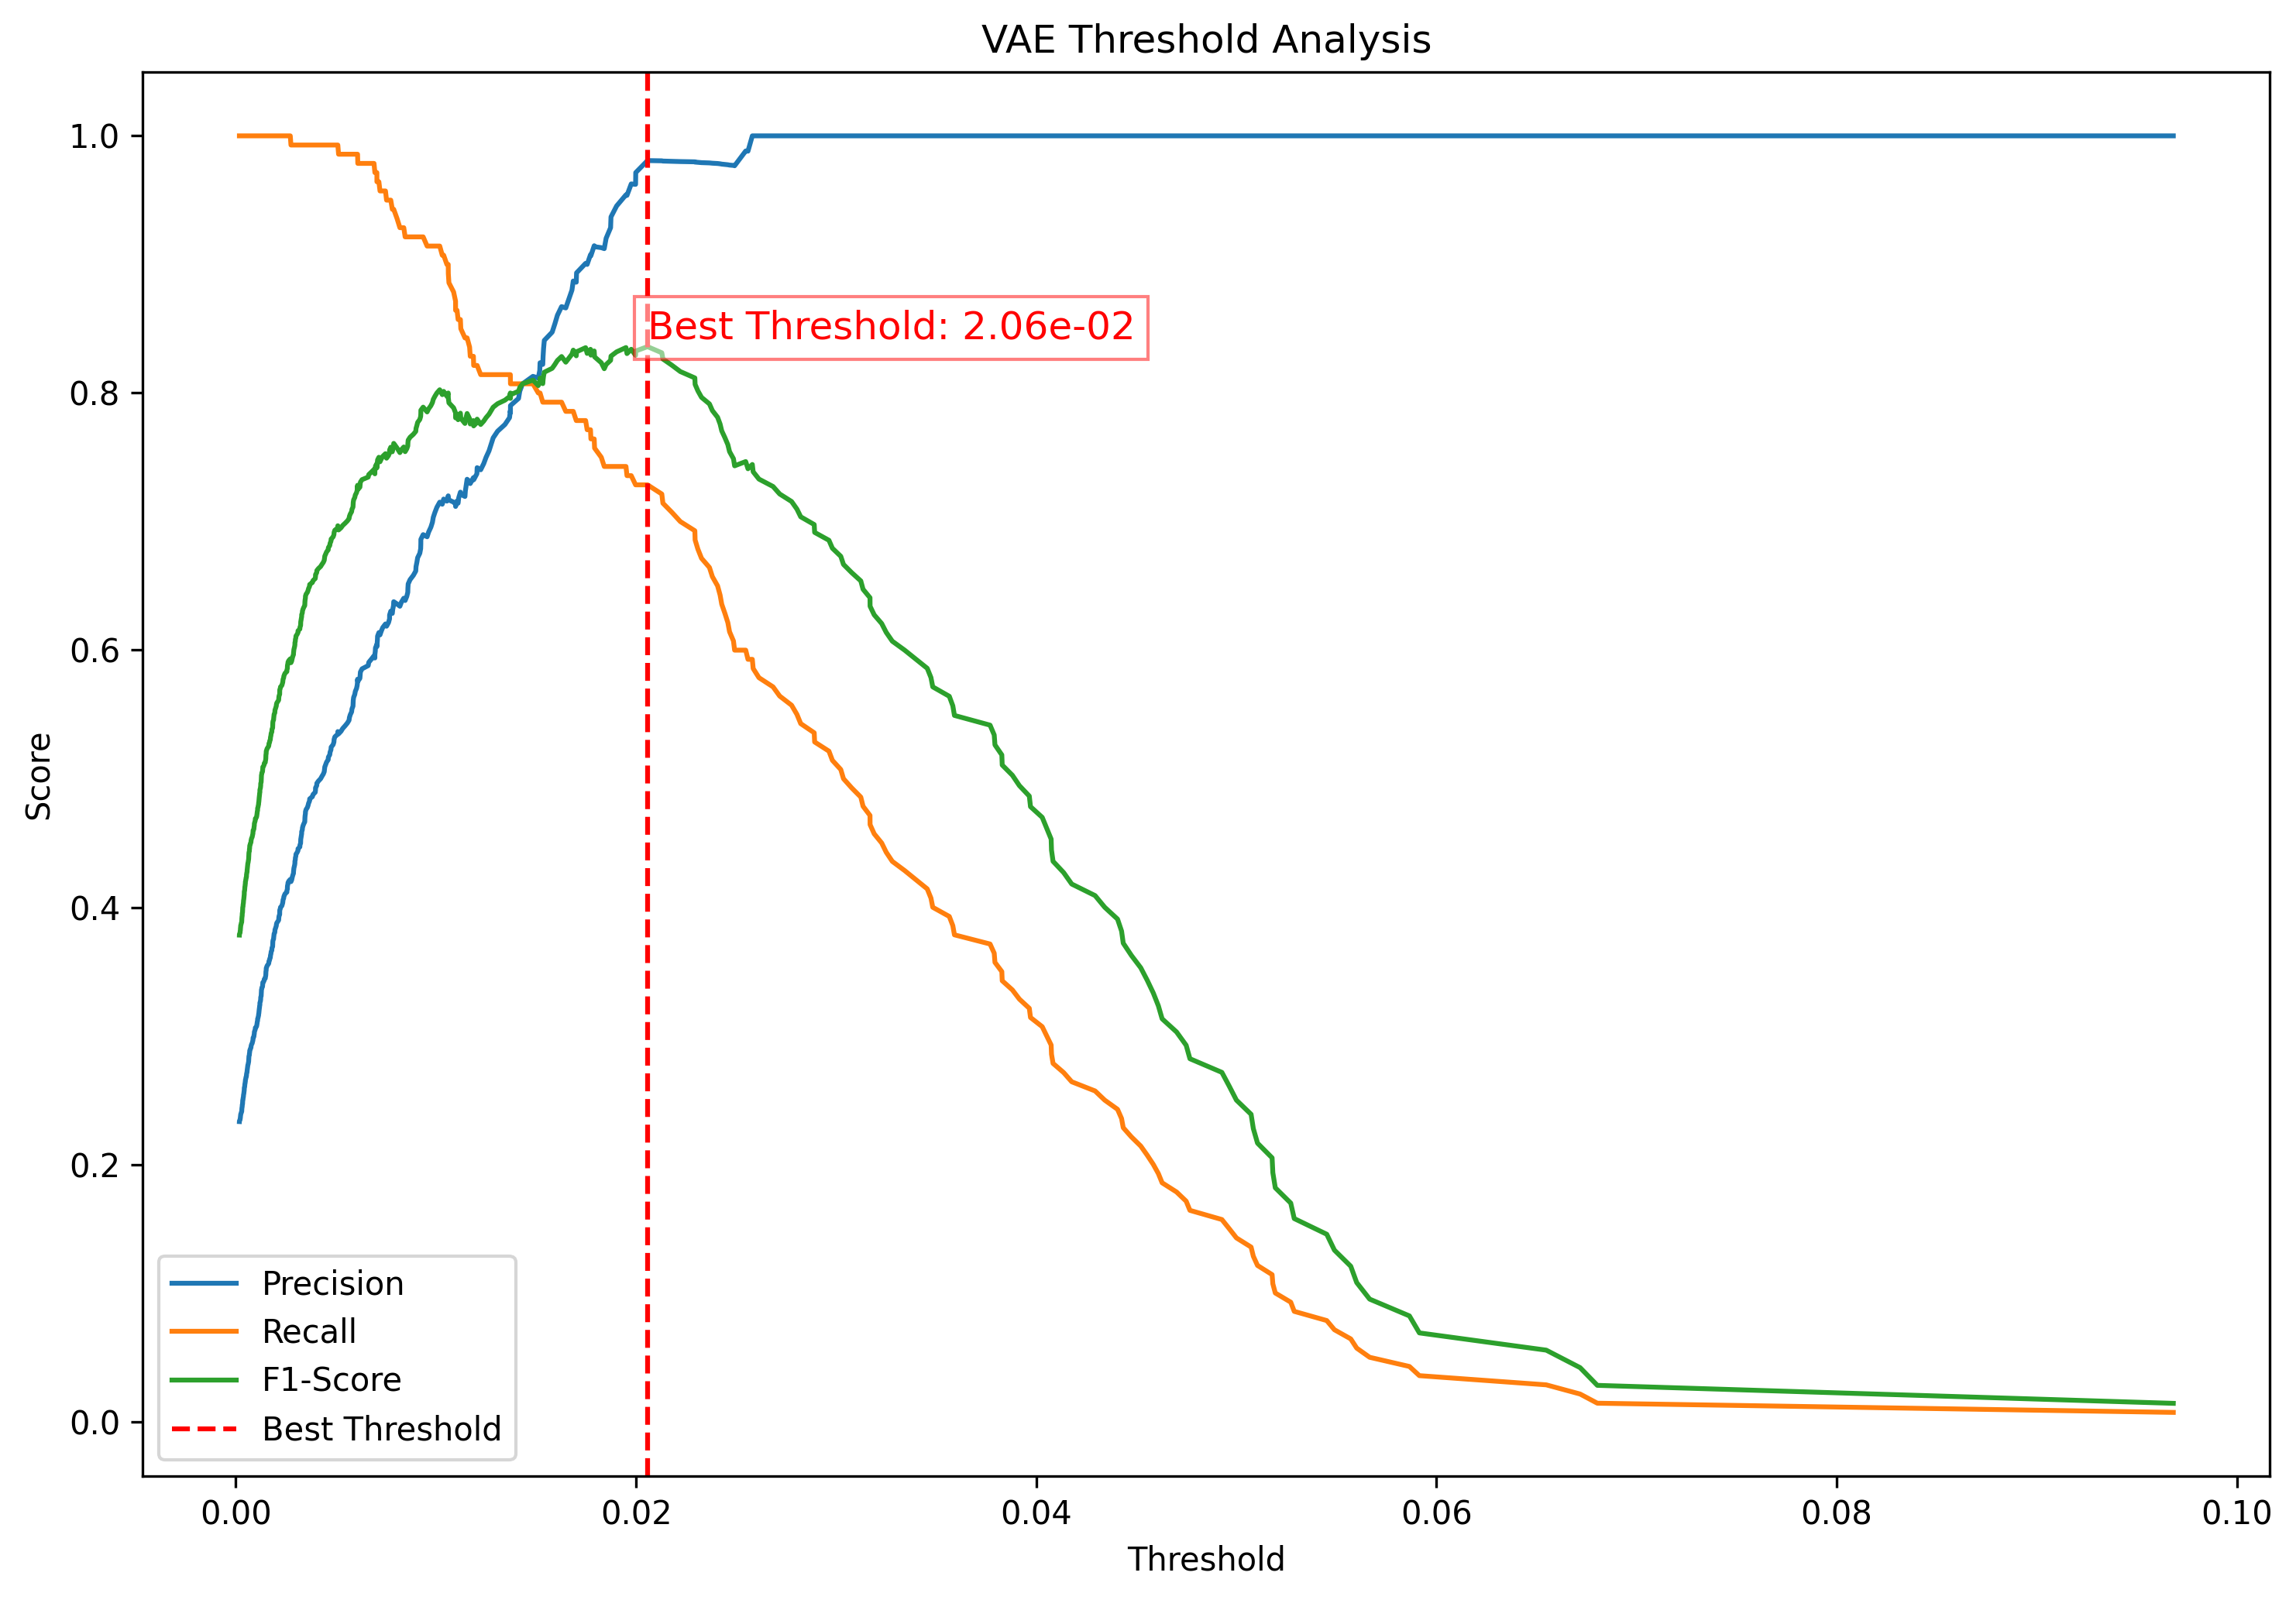
\includegraphics[scale=0.5]{figures/anomalies/vae/threshold.png}
  \caption{$\beta$-VAE}
  \label{fig:threshold_vae}
\end{figure}

\begin{figure}[!h]
  \centering
  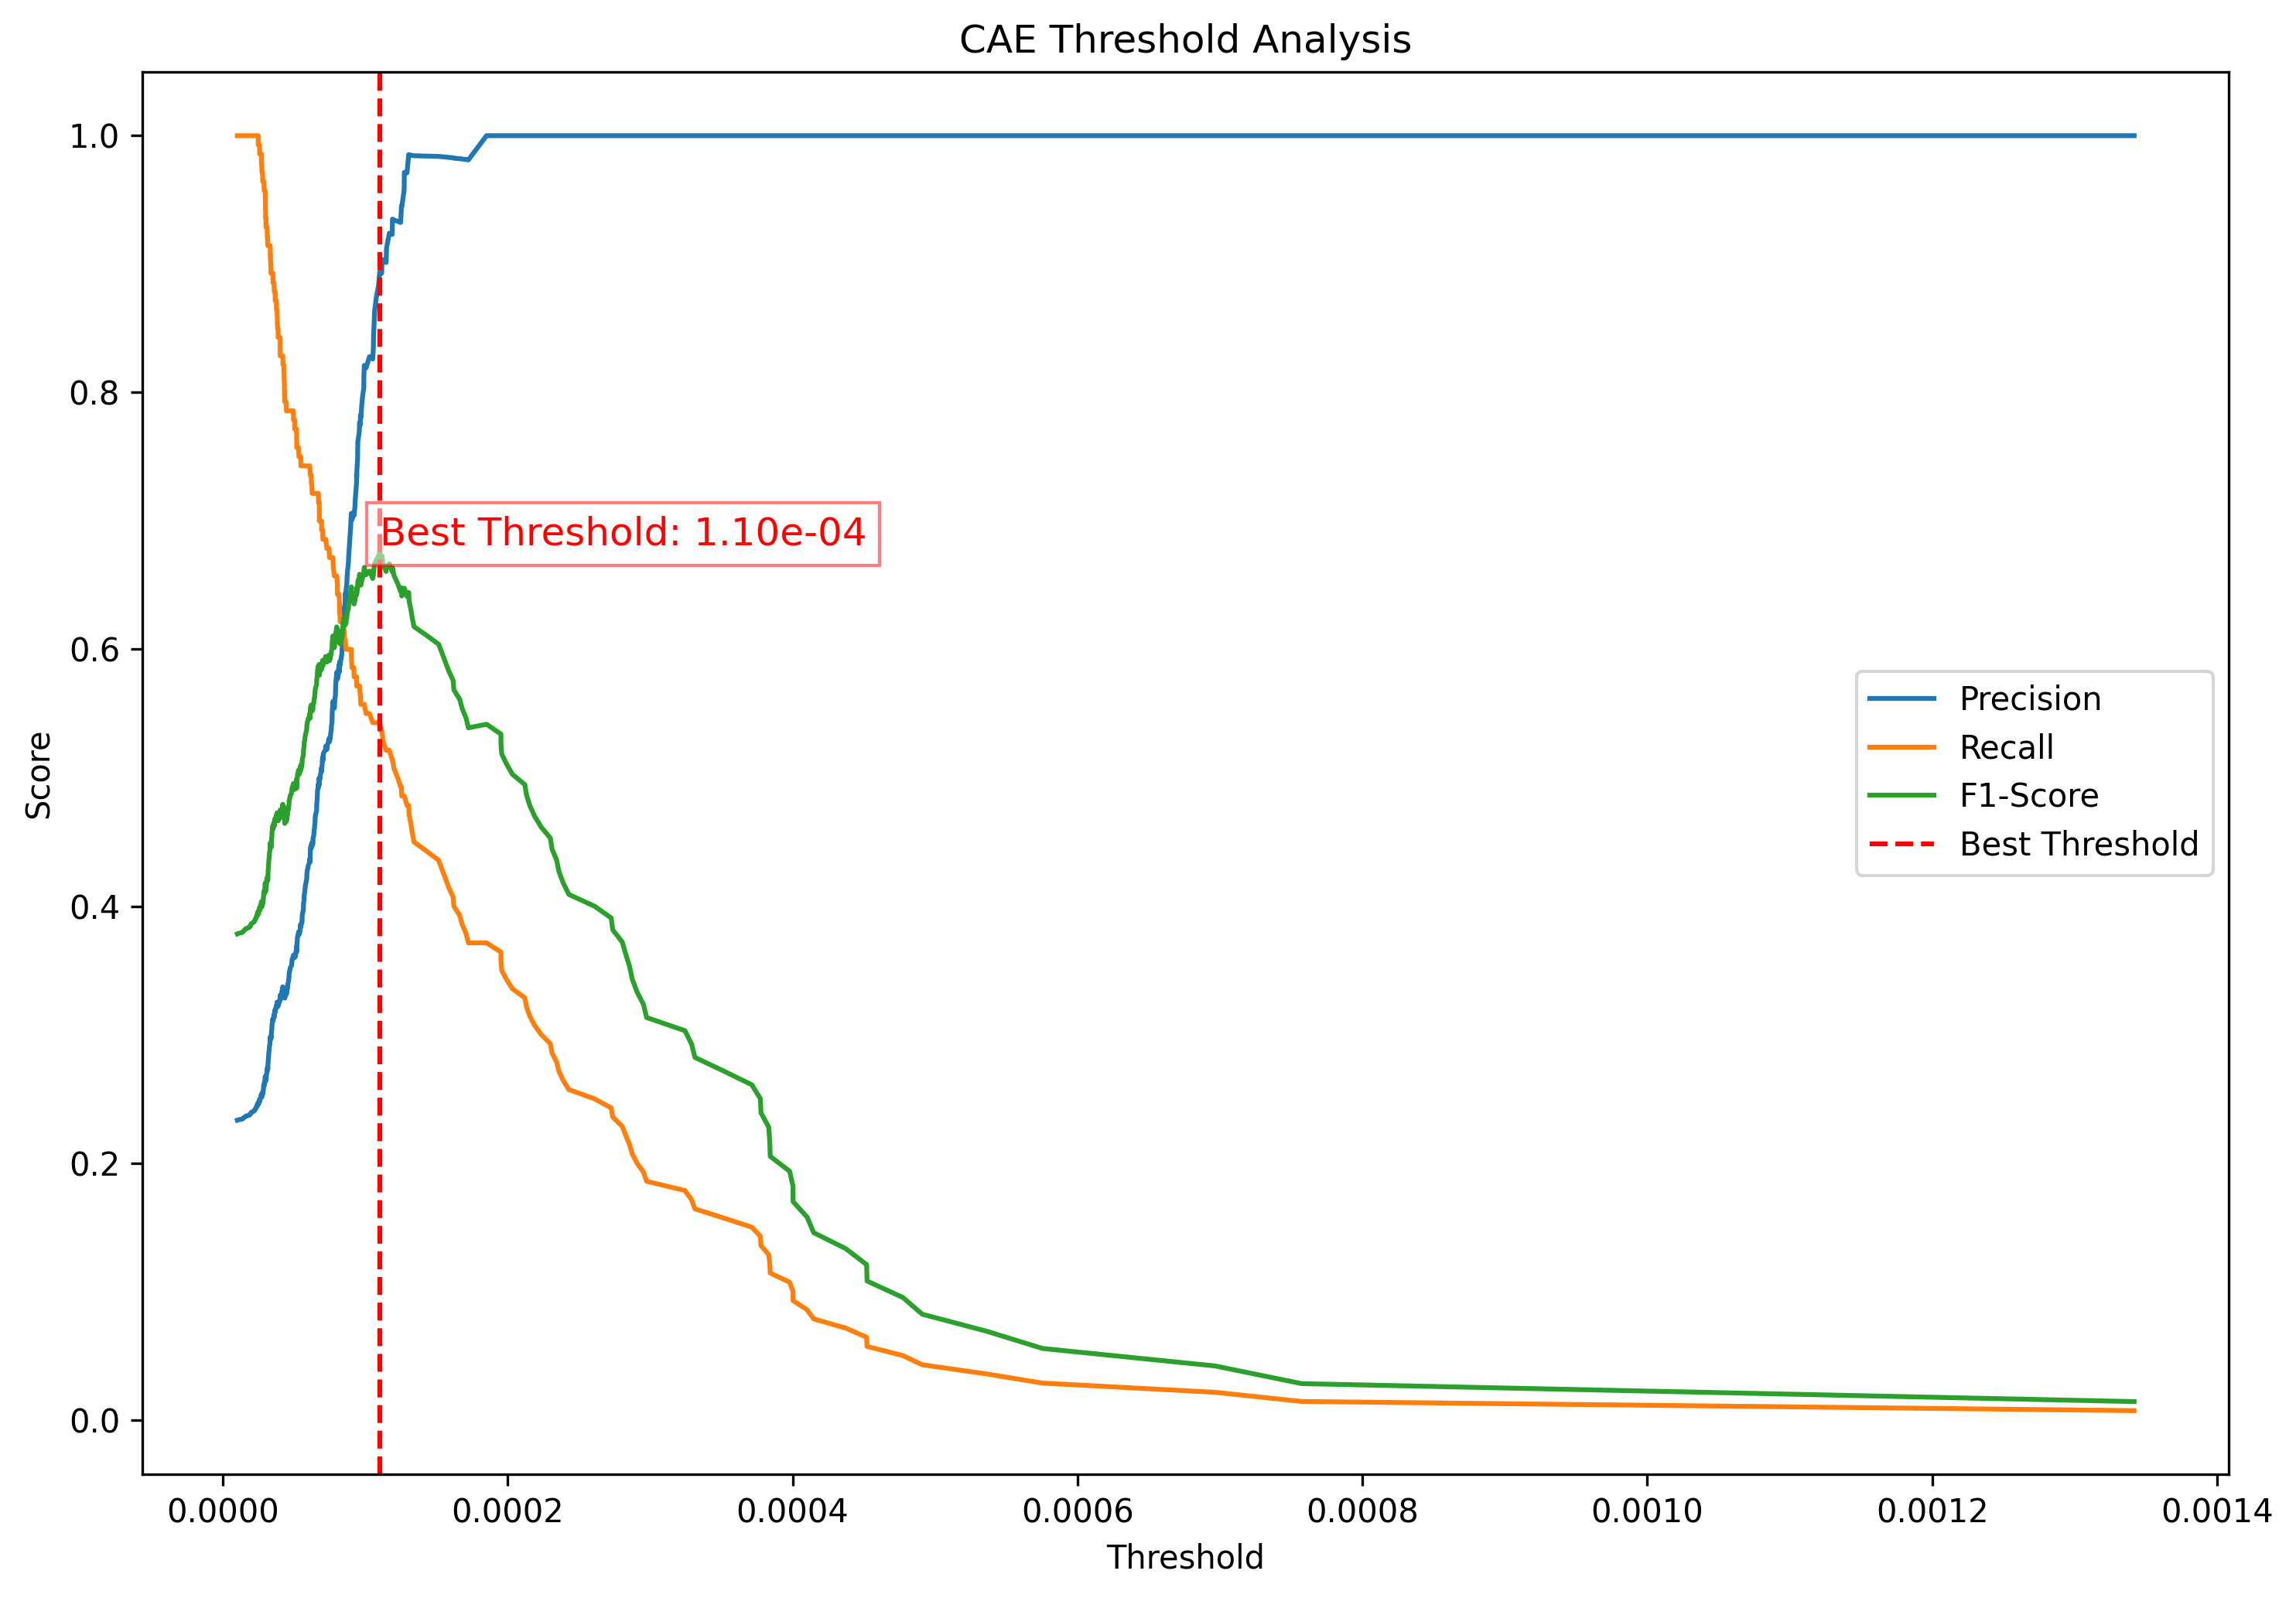
\includegraphics[scale=0.5]{figures/anomalies/cae/threshold.png}
  \caption{CAE}
  \label{fig:threshold_cae}
\end{figure}

\begin{figure}[!h]
  \centering
  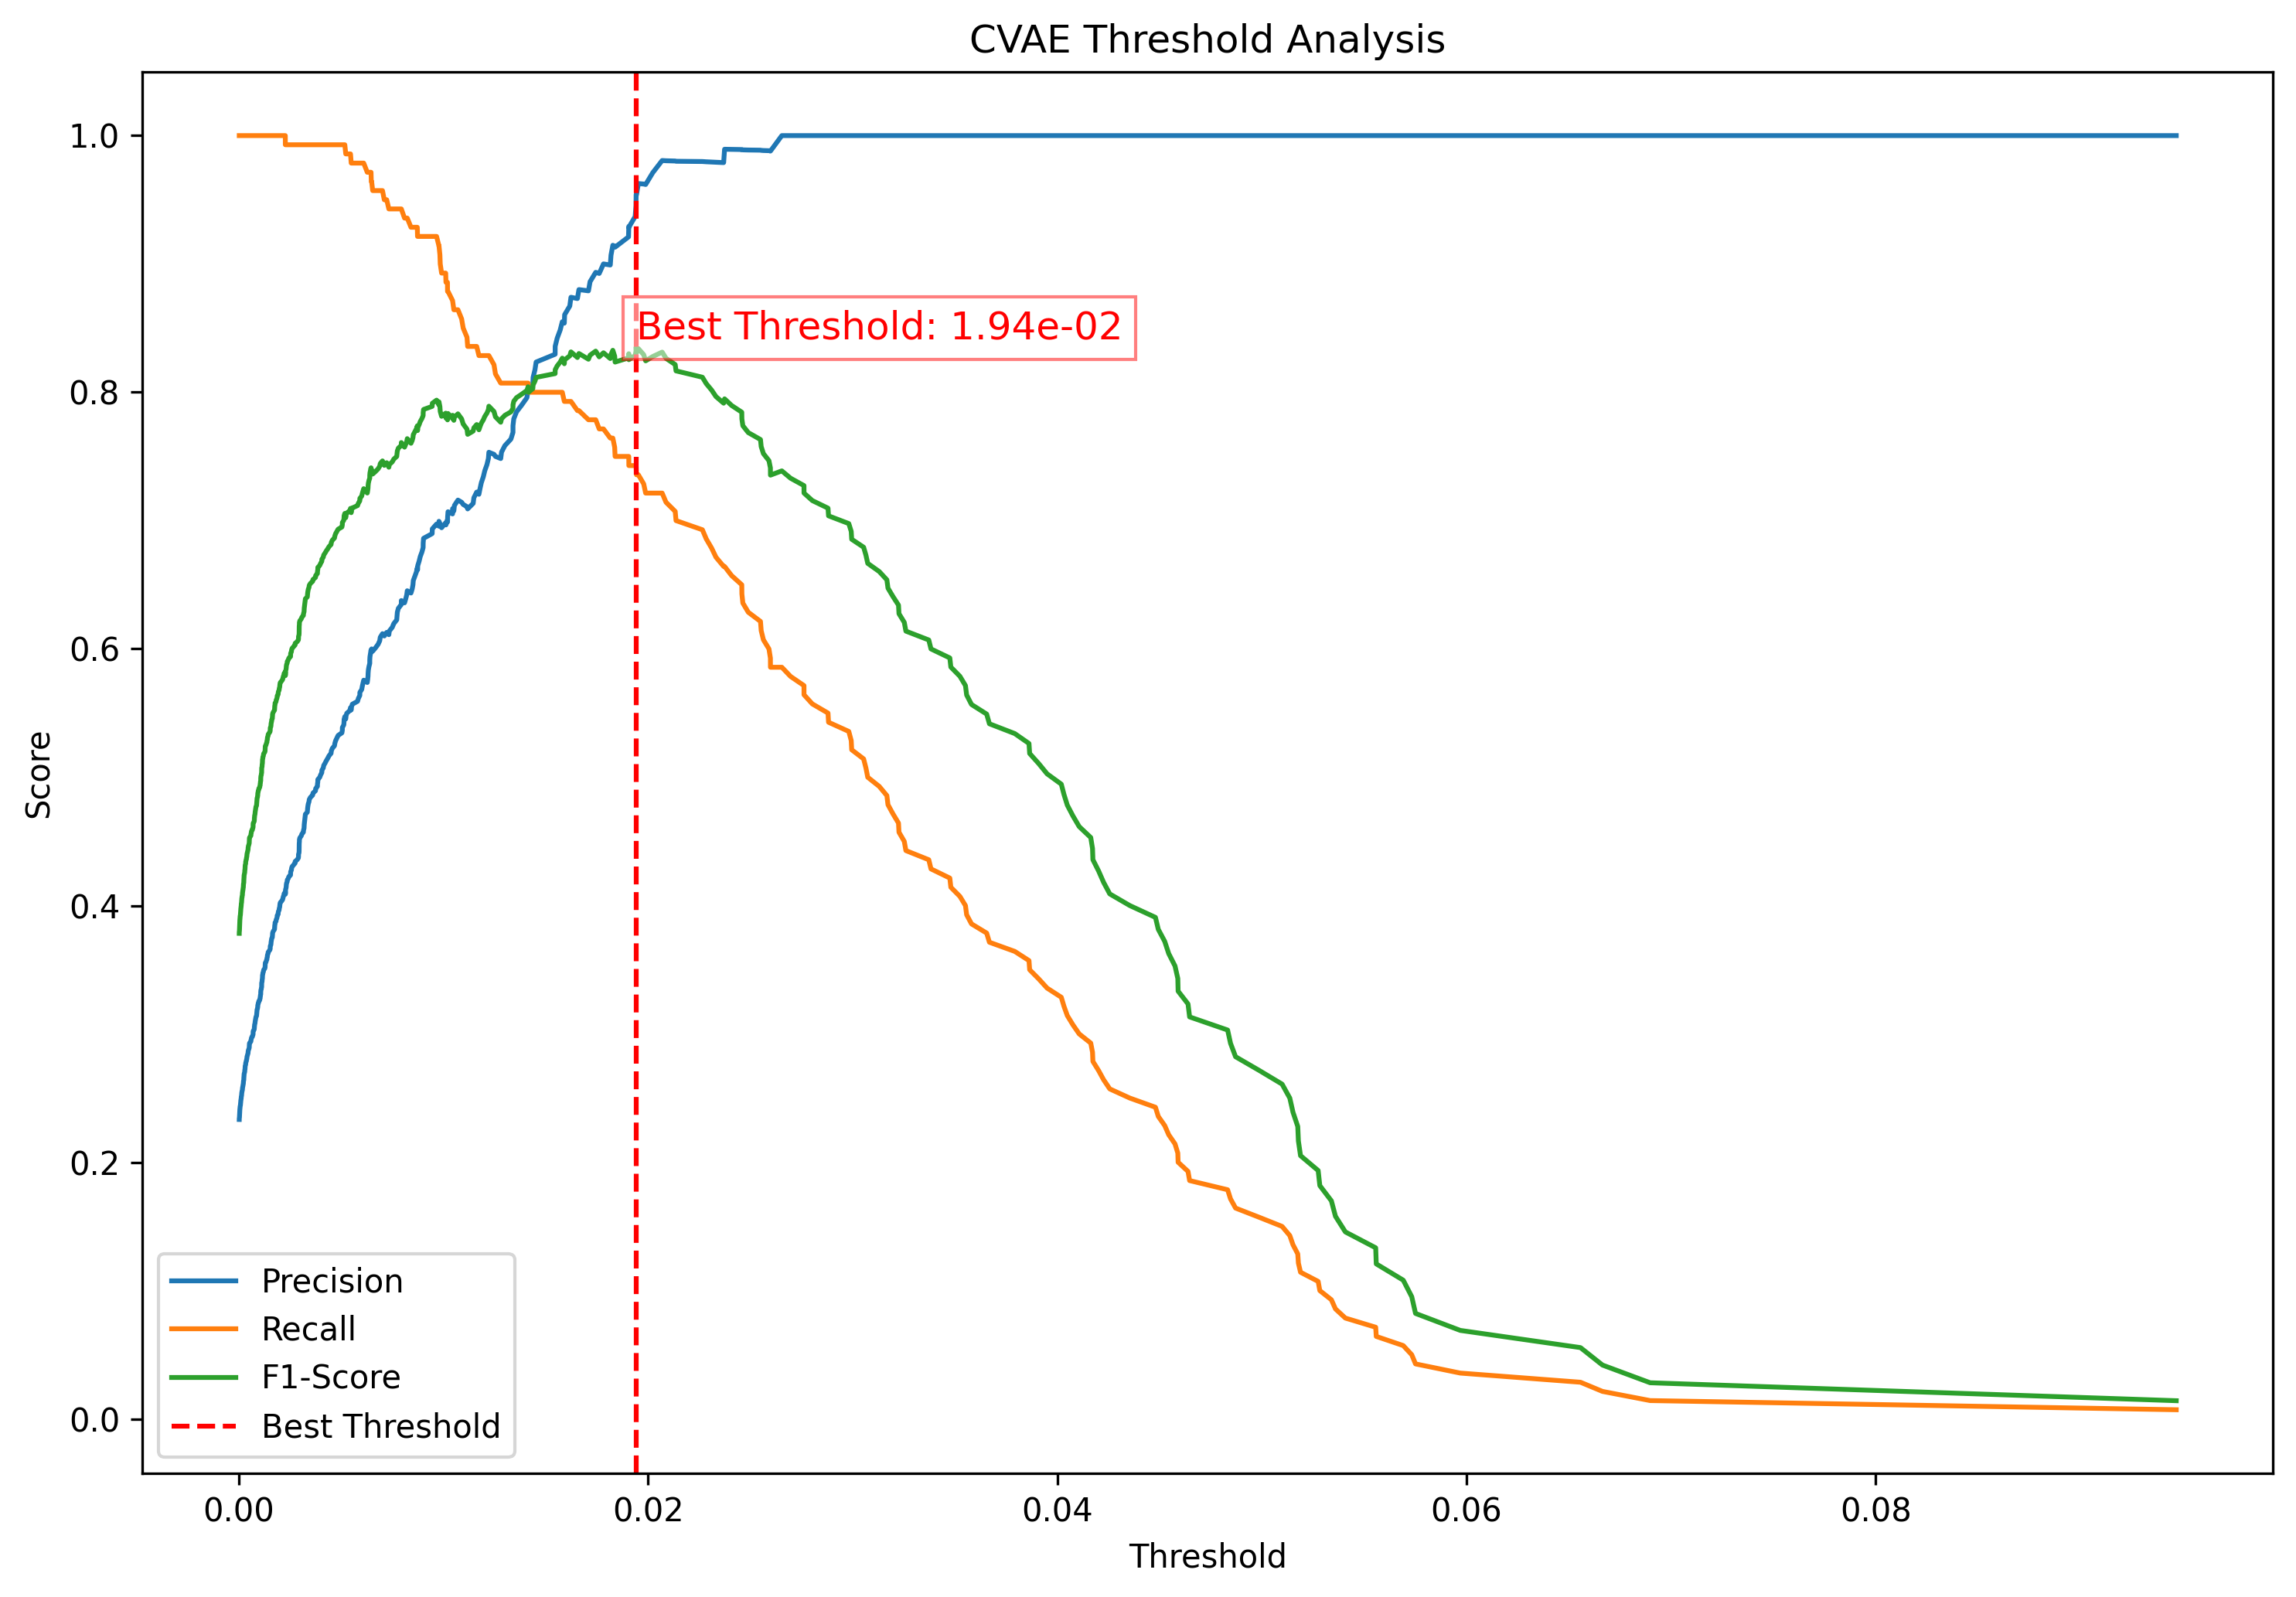
\includegraphics[scale=0.5]{figures/anomalies/cvae/threshold.png}
  \caption{$\beta$-CVAE}
  \label{fig:threshold_vae}
\end{figure}
